\documentclass[12pt]{article}
\usepackage{common}
\setlength{\parindent}{0in}
\renewcommand\arraystretch{1.9}
\newcommand{\un}{\ensuremath{\hat{U}_{N\sigma}}}
\newcommand{\no}{\ensuremath{\hat{n}_{N\sigma}}}
\newcommand{\hml}{\ensuremath{\ham_{2N}}}
\begin{document}
\begin{titlepage}
\begin{center}
	\vspace{10pt}
\bf{\Huge{Unitary Renormalization Group Approach to the Hubbard Dimer and Anderson Molecule}}\\
	\vspace{50pt}
\end{center}

\end{titlepage}

\section*{Abstract}
The power of exact analytical methods over numerical or approximate methods is that they give more comprehensive answers and explanations. Take for example the difference between a wavefunction obtained from exact diagonalization and a plot of the wavefunction obtained from numerical analysis. While the latter gives you an idea, the former gives you the complete thing. In this report, I follow a similar theme: I explore an exact method in a condensed matter setting. This exact method (a unitary renormalization group method) is used to solve two toy models - the Hubbard dimer and Anderson molecule). The focus is to showcase this method rather than learning about the models, because the models are exactly diagonalizable anyway. It is seen that the solutions the URG match exactly with the exact diagonalization results. A comparison is also drawn with a similar block-diagonalization method- the Schrieffer-Wolff transformation. It is seen that while the SW transformation is perturbative and one must truncate the expansion at some point to get something out of it, the URG is exact.
\newpage

\tableofcontents

\newpage
\section{Introduction}
Condensed matter physics is mostly many-body in nature, and usually deals with huge number of particles. As such, it is usually not possible to obtain exact solutions to problems, and one usually resorts to approximate methods such as perturbative techniques or numerical solutions. The problem with such methods is that they do not always work, some problems might require exact solutions and it is always more appealing to get exact solutions compared to approximate ones. Taking this thread, Anirban Mukherjee in Dr. Siddhartha Lal's group devised an algorithm to unitarily rotate the Hamiltonian progressively into a block-diagonalized form, hence obtaining the eigenvalues and eigenvectors of the problem.
\paragraph{}
The way this algorithm works is the following: first a particular degree of freedom of the problem is chosen. This degree of freedom is then decoupled from the problem by block-diagonalization  the Hamiltonian in the subspace of this degree of freedom. This is achieved by considering transition operators that take states from the occupied part of this degree of freedom to the unoccupied part and vice-versa. These operators are shown to have certain properties which involve the block-diagonal parts of the Hamiltonian. By using these properties (that is, the equations obtained thereof), these block-diagonal parts can be extracted. Once these parts are extracted, the Hamiltonian is block-diagonal in this degree of freedom, and this can be done recursively to diagonalize the whole Hamiltonian.
\paragraph{}
This method has already been applied by Anirban Mukherjee and others in the group to study several problems. The most notable among these is an exact solution of the two-dimensional Hubbard model at half-filling for zero temperature. Since this method is relatively new, my motivation in this project was to get a better feel for this method by solving two models which can be exactly diagonalised, namely the two site Hubbard model and the two site Anderson model. Since the exact solutions of these models are available, the approach via the renormalization group method can be compared with the exact diagonalization process, leading to a better understanding of the process. A similar approach in this respect is the Schrieffer-Wolff transformation; it also seeks to block-diagonalize the Hamiltonian. Hence it makes sense to draw a comparison between the two methods. The models are analysed using the Schrieffer-Wolff transformation, and the differences between the approaches are noted.
\paragraph{}
Since this method uses the properties of the Fermionic creation and annihilation operators, this method can be used only on Fermionic Hamiltonians. In the first sections, I solve the two models using exact diagonalization. The first model is the Hubbard dimer. It consists of two lattice sites, with hopping between them parameterised by a hopping strength \il{t}, and an on-site repulsion for both sites, parameterised by \il{U}. This Hamiltonian is solved by making use of the symmetries of the system: the total number operator \il{\hat n = \sum_{i,\sigma} n_{i\sigma}}, the total magnetization operator \il{\hat S_z = \sum_{i}(n_{i\ua}-n_{i\da})} and the site parity operator \il{\hat P: c_1 \leftrightarrow c_2} commute with the Hamlitonian. These commutations are proved, and then used to diagonalize the Hamiltonian in the subspace of the eigenstates of the operators. Similarly, the Anderson molecule is a two site version of the Anderson impurity model. One site represents the d-orbital impurity site, with site energy \il{\epsilon_d}, and the other site represents the conduction band, with energy (and hence chemical potential, because there is just the one conduction band electron) \il{\epsilon_s}. There is hopping between them, with strength \il{t}, and an on-site repulsion on the impurity site only, with a penalty of \il{U}. This model is also solved similar to the Hubbard dimer, by making use of the symmetries. After solving the models, I show that they lead to other models in limit of high \il{U}: the Hubbard dimer goes to the Mott insulator and the Anderson molecule goes to the Kondo molecule.

\paragraph{}
Next, I derive the formalism of the unitary renormalization group method used here. Starting from a general Fermionic Hamiltonian, a transition operator \il{\eta} is defined, and the block-diagonalized Hamiltonian is found to obey certain relations. These relations will ultimately be used to block diagonalize the Hamiltonians. I apply the URG both in position and momentum space. The results match with the ones obtained from exact diagonalization, because the URG uses unitary rotations which should keep the eigenvalues and vectors intact. Finally, I show the method of Schrieffer-Wolff transformation very briefly on both the models, focussing on the changes made to the Hamiltonian along the way. The changes are in some sense similar since both the methods (SW and URG) strive to block-diagonalise the Hamiltonian, but the SW transformation enforces the limit of large \il{U}, because only terms up to second order are kept, otherwise the method is not tractable, while the URG does not drop any order.

\newpage
\section{Exact diagonalization of the Hubbard dimer (real space)}

\pp[The Hamiltonian]
\beq
\ham = -t\sum_\sigma\rr{\C{1}{\sigma}\c{2}{\sigma}+\C{2}{\sigma}\c{1}{\sigma}} + U\sum_i\hat{n}_{i\uparrow}\hat{n}_{i\downarrow}
\eeq
I have 2 lattice sites, indexed by 1 and 2, occupied by electrons. \C{i}{\sigma} and \(c_{i\sigma}\) are the fermionic creation and annihilation operators at the i\uu{th} site, with spin-index \(\sigma\). \(\sigma\) can take values \(\uparrow\) and \(\downarrow\), denoting spin-up and spin-down states respectively. \(\hat{n}_{i\sigma}=\C{i}{\sigma} \c{i}{\sigma}\) is the number operator for the \(i^{th}\) site and at spin-index \(\sigma\); it counts the number of fermions with the designated quantum numbers.  \it t is the hopping strength; the more the t, the more are the electrons likely to hop between sites. \it U is the on-site repulsion cost; it represents the penalty incurred in energy when two electrons occupy the same site.

\subsection{Symmetries of the problem}
The following operators commute with the Hamiltonian.
\begin{enumerate}
\item\bf{Total number operator}: \(\qq{\ham, \hat N}=0\).
\begin{proof}
The last term in the Hamiltonian is the number operator itself. Ignoring that, there are three terms that I need to individually consider.
\begin{itemize}
\item \(\C{1}{\sigma}\c{2}{\sigma}\)
\beq[commutator]
\qq{\C{1}{\sigma}\c{2}{\sigma},\hat{n}_{i\sigma^\prime}} &= \qq{\C{1}{\sigma}\c{2}{\sigma},\C{i}{\sigma^\prime}\c{i}{\sigma^\prime}} \\
&= \C{1}{\sigma} \qq{\c{2}{\sigma},\C{i}{\sigma^\prime}\c{i}{\sigma^\prime}}+\qq{\C{1}{\sigma},\C{i}{\sigma^\prime}\c{i}{\sigma^\prime}}\c{2}{\sigma} \\
&= \delta_{i,2}\:\C{1}{\sigma} \qq{\c{2}{\sigma},\C{2}{\sigma^\prime}\c{2}{\sigma^\prime}}+\delta_{i,1}\qq{\C{1}{\sigma},\C{1}{\sigma^\prime}\c{1}{\sigma^\prime}}\c{2}{\sigma} \\
&= \delta_{i,2}\:\C{1}{\sigma} \cc{\c{2}{\sigma},\C{2}{\sigma^\prime}}\c{2}{\sigma^\prime} - \delta_{i,1}\C{1}{\sigma^\prime}\cc{\c{1}{\sigma^\prime},\C{1}{\sigma}}\c{2}{\sigma} \\
&= \delta_{\sigma,\sigma^\prime}\C{1}{\sigma}\c{1}{\sigma}\rr{\delta_{i,2} - \delta_{i,1}}
\eeq
The third line follows because the electrons on different sites are distinguishable and hence, the \it{creation and annihilationihilation operators of different sites will commute among themselves}. Therefore,
\beq
\qq{\C{1}{\sigma}\c{2}{\sigma}, \hat{N}} &= \sum_{i\sigma^\prime}\qq{\C{1}{\sigma}\c{2}{\sigma},\hat{n}_{i\sigma^\prime}} = \C{1}{\sigma}\c{1}{\sigma}\sum_{i=\{1,2\}}\rr{\delta_{i,2} - \delta_{i,1}} = 0
\eeq

\item \(\C{2}{\sigma}\c{1}{\sigma}\): Since the operator \(\hat{N}\) is symmetric with respect to the site indices 1 and 2, I can go through the last proof again with the site indices 1 and 2 exchanged and since the proof does not depend on the site indices, this commutator will also be zero.

\item \(\hat{n}_{i\uparrow}\hat{n}_{i\downarrow}\):
\beq[commutator_2]
\qq{\hat{n}_{i\uparrow}\hat{n}_{j\downarrow},\hat{n}_{j\sigma}} &= \hat{n}_{i\uparrow}\qq{\hat{n}_{i\downarrow},\hat{n}_{j\sigma}} - \qq{\hat{n}_{i\uparrow},\hat{n}_{j\sigma}}\hat{n}_{i\downarrow} \\
&= \delta_{ij}\rr{\hat{n}_{i\uparrow}\qq{\hat{n}_{i\downarrow},\hat{n}_{i\sigma}} - \qq{\hat{n}_{i\uparrow},\hat{n}_{i\sigma}}\hat{n}_{i\downarrow}} \\
&= \delta_{ij}\rr{\delta_{\sigma\uparrow}\hat{n}_{i\uparrow}\qq{\hat{n}_{i\downarrow},\hat{n}_{i\uparrow}} - \delta_{\sigma\downarrow}\qq{\hat{n}_{i\uparrow},\hat{n}_{i\downarrow}}\hat{n}_{i\downarrow}} \\
&= \delta_{ij} \rr{\delta_{\sigma\downarrow}\hat{n}_{i\downarrow} - \delta_{\sigma\uparrow}\hat{n}_{i\uparrow}} \qq{\hat{n}_{i\uparrow},\hat{n}_{i\downarrow}} \\
&= \delta_{ij} \rr{\delta_{\sigma\downarrow}\hat{n}_{i\downarrow} - \delta_{\sigma\uparrow}\hat{n}_{i\uparrow}} \rr{\C{i}{\uparrow}\c{i}{\uparrow}\C{i}{\downarrow}\c{i}{\downarrow}-\C{i}{\downarrow}\c{i}{\downarrow}\C{i}{\uparrow}\c{i}{\uparrow}}\\
&= \delta_{ij} \rr{\delta_{\sigma\downarrow}\hat{n}_{i\downarrow} - \delta_{\sigma\uparrow}\hat{n}_{i\uparrow}} \rr{\C{i}{\downarrow}\c{i}{\downarrow}\C{i}{\uparrow}\c{i}{\uparrow}-\C{i}{\downarrow}\c{i}{\downarrow}\C{i}{\uparrow}\c{i}{\uparrow}} = 0
\eeq
Therefore, \(\qq{\hat{n}_{i\uparrow}\hat{n}_{j\downarrow},\hat{N}} = \sum_{j,\sigma} \qq{\hat{n}_{i\uparrow}\hat{n}_{j\downarrow},\hat{n}_{j\sigma}} = 0\)
% \beq
% \qq{\hat{n}_{i\uparrow}\hat{n}_{i\downarrow}, \hat{N}} &= \sum_{j\sigma}\qq{\hat{n}_{i\uparrow}\hat{n}_{j\downarrow},\hat{n}_{j\sigma}} \\
% &= \sum_{\sigma}\qq{\hat{n}_{i\uparrow}\hat{n}_{i\downarrow},\hat{n}_{i\sigma}} \\
% &= \hat{n}_{i\uparrow}\qq{\hat{n}_{i\downarrow},\hat{n}_{i\uparrow}}+\qq{\hat{n}_{i\uparrow},\hat{n}_{i\downarrow}}\hat{n}_{i\downarrow} = 0
% \eeq

\end{itemize}
The total Hamiltonian is just a sum of the three terms; since the number operator commutes individually with these terms, it obviously commutes with the total Hamiltonian.
\end{proof}
\item \bf{Magnetization operator}: \(\hat{S}^z_{tot} \equiv \frac{1}{2}\sum_i\rr{\hat{n}_{i\uparrow}-\hat{n}_{i\downarrow}}\), \(\qq{\ham, \hat{S}^z_{tot}}=0\).
\begin{proof}
The magnetization operator can be rewritten as \(\hat{S}^z_{tot} = \frac{1}{2}\sum_i\rr{\hat{n}_{i\uparrow}+\hat{n}_{i\downarrow}-2\hat{n}_{i\downarrow}} = \hat{N} - 2\sum_i\hat{n}_{i\downarrow}\). Since \(\hat{N}\) commutes with \(\ham\), I just need to prove that \(\qq{\ham, \sum_i\hat{n}_{i\downarrow}}\). From eq. \ref{commutator}, 
\beq
\qq{\C{1}{\sigma}\c{2}{\sigma},\sum_i\hat{n}_{i\downarrow}} &= \C{1}{\downarrow}\c{1}{\downarrow}\sum_{i=\{1,2\}}\rr{\delta_{i,2} - \delta_{i,1}} = 0
\eeq
Again using the symmetry of the magnetization operator with the exchange of indices, its obvious that
\qq{\C{2}{\sigma}\c{1}{\sigma},\sum_i\hat{n}_{i\downarrow}} = 0

Using eq. \ref{commutator_2}, \(\qq{\hat{n}_{i\uparrow}\hat{n}_{i\downarrow}, \hat{n}_{i\downarrow}} = 0\).

Finally, \(\qq{N, \hat{n}_{i\downarrow}}=\sum_{j\sigma}\qq{\hat{n}_{j\sigma},\hat{n}_{i\downarrow}} = \qq{\hat{n}_{i\uparrow},\hat{n}_{i\downarrow}} = \C{i}{\uparrow}\c{i}{\uparrow}\C{i}{\downarrow}\c{i}{\downarrow}-\C{i}{\downarrow}\c{i}{\downarrow}\C{i}{\uparrow}\c{i}{\uparrow} = 0\). Since \(\hat{S}^z_{tot}\) commutes with each part individually, it commutes with the total Hamiltonian.
\end{proof}

\item \bf{Two-site parity operator \(\hat{P}\)}: The action of \(\hat{P}\) is defined as follows. If \(\ket{\Psi_{\alpha\beta}}\) is a wavefunction with site indices \(\alpha\) and \(\beta\), 
\beq
\hat{P}\ket{\Psi(\alpha,\beta)} = \ket{\Psi(\beta,\alpha)}
\eeq
That is, it operates on each electron and reverses it's site indices. 
\begin{proof}
I now rewrite the Hamiltonian by explcitly showing the two site indices:
\beq
\ham(\alpha,\beta) = -t\sum_\sigma(\C{\alpha}{\sigma}\c{\beta}{\sigma}+\C{\beta}{\sigma}\c{\alpha}{\sigma}) + U(n_{\alpha\uparrow}n_{\alpha\downarrow}+n_{\beta\uparrow}n_{\beta\downarrow}) - \mu\sum_\sigma(n_{\alpha\sigma}+n_{\beta\sigma})
\eeq 
Its obvious that \(\ham\) is symmetric in the site indices: \(\ham(\alpha,\beta) = \ham(\beta,\alpha)\). This means that the eigenvalues also have this symmetry. Let \(\ket{\Phi(\alpha,\beta)}\) be an eigenstate of \(\ham(\alpha,\beta)\) with eigenvalue \(E(\alpha,\beta)\). Then,
\beq
\hat{P}\ham\ket{\Phi(\alpha,\beta)} &= E(\alpha,\beta) \hat{P}\ket{\Phi(\alpha,\beta)} = E(\beta,\alpha) \ket{\Phi(\beta,\alpha)} \\
&= \ham \ket{\Phi(\beta,\alpha)} = \ham \hat{P} \ket{\Phi(\alpha,\beta)} \\
\implies \ham\hat{P}\ket{\Phi(\alpha,\beta)} &= \hat{P}\ham\ket{\Phi(\alpha,\beta)}
\eeq
Since any general wavefunction can be expanded in terms of these wavefunctions and since both the operator are linear, the above result will also hold for a general wavefunction \(\ket{\Psi(\alpha,\beta)}\):
\beq
\ham \hat{P} \ket{\Psi(\alpha,\beta)} = \hat{P} \ham \ket{\Psi(\alpha,\beta)}
\implies [\ham, \hat{P}] = 0
\eeq
\end{proof}
\end{enumerate}
\subsection{Partitioning the Hilbert space}

The Hamiltonian commutes with the three operators. This means that is possible to simultaneously diagonalize these four operators: \(\ham, \hat{N}, S_z^{tot}, \hat{P}\). I will be able to label the eigenstates of the total Hamiltonian using the eigenvalues of these operators. First take the total number operator. \(\hat{N}\) can take four values for a two-site system, 1 through 4. The eigenstates labelled by a particular number, say N=2 will be orthogonal to the eigenstates labelled by another number, say N=4. This means each eigenvalue of \(\hat{N}\) will have a distinct subspace orthogonal to the other values of \(\hat{N}\). I will be able to diagonalize each such subspace independently of each other, because they will not have any overlap. This feature enables us to block-diagonalize the total Hamiltonian into four blocks, each block belonging to each value \(\hat{N}\). 

\paragraph{}
Inside each block, I will be able to repeat the procedure by next using the eigenvalues of \(S_z^{tot}\). Each block of the Hamiltonian will again break up to smaller blocks for each value of the total magnetization. The eigenvalues of parity operator provide a further partitioning of the blocks of magnetization. For writing the state kets, I use the following notation: \(\ket{\uparrow,\downarrow}\) means electron on site 1 has spin up and that on site 2 has spin-down. \(\ket{\downarrow, 0}\) means electron on site 1 has spin-down and there is no electron on site 2.

\subsection{N = 1}

\pp For one electron on two lattice sites, I start by writing down the eigenstates of \(S_z^{tot}\). For odd number of electrons, zero magnetization is not possible. 
\begin{center}
	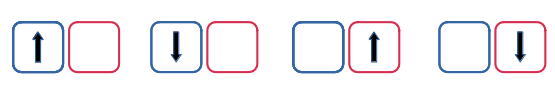
\includegraphics[scale=0.5]{one.png}
\end{center}
So,
\begin{itemize}
	\item[$\ast$] \(S_z^{tot} = -1\): \(\ket{\downarrow,0}, \ket{0, \downarrow}\)
	\item[$\ast$] \(S_z^{tot} = +1\): \(\ket{\uparrow,0}, \ket{0, \uparrow}\)
\end{itemize}
Each eigenvalue will have a separate subspace and can be separately diagonalized. I need to find the matrix elements of \(\ham\) in these eigenkets. Since there is no possibility of two electrons occupying same site, I ignore the \(U\)-term for the time being.

\begin{itemize}

\item{\(S_z^{tot} = -1\)}
Let us first see the action of the Hamiltonian on the eigenfunctions with \(S_z^{tot} = -1\).
\beq
\ham\ket{\downarrow,0} = -t \C{2}{\downarrow}\c{1}{\downarrow}\ket{\downarrow,0} = -t\ket{0,\downarrow} \\
\ham\ket{0,\downarrow} = -t \C{1}{\downarrow}\c{2}{\downarrow}\ket{0,\downarrow} = -t\ket{\downarrow,0} \\
\eeq
We get the following matrix for this tiny subspace of the Hamiltonian:
\beq
\bordermatrix{~ & \ket{\downarrow,0} & \ket{0,\downarrow} \cr
              \ket{\downarrow,0} & 0 & -t \cr \\
              \ket{0,\downarrow} & -t & 0 \cr}
\eeq

The eigenvalues and eigenvectors of this matrix are \(\frac{\ket{\downarrow,0} \pm \ket{0,\downarrow}}{\sqrt{2}}\), with eigenvalues \(\mp t\). These are also the eigenvalues of the parity operator, as expected.
\beq
\hat{P}\rr{\ket{\downarrow,0} + \ket{0,\downarrow}} = \ket{0,\downarrow} + \ket{\downarrow,0} \implies \hat{P} = 1 \\
\hat{P}\rr{\ket{\downarrow,0} - \ket{0,\downarrow}} = \ket{0,\downarrow} - \ket{\downarrow,0} \implies \hat{P} = -1
\eeq

\item{\(S_z^{tot} = +1\)}
Now I look at the spin-up states.
\beq
\ham\ket{\uparrow,0} = -t \C{2}{\uparrow}\c{1}{\uparrow}\ket{\uparrow,0} = -t\ket{0,\uparrow} \\
\ham\ket{0,\uparrow} = -t \C{1}{\uparrow}\c{2}{\uparrow}\ket{0,\uparrow} = -t\ket{\uparrow,0} \\
\eeq
Clearly, this gives the same matrix as the spin-down states:
\beq
\bordermatrix{~ & \ket{\uparrow,0} & \ket{0,\uparrow} \cr
              \ket{\uparrow,0} & 0 & -t \cr \\
              \ket{0,\uparrow} & -t & 0 \cr}
\eeq
and hence similar eigenfunctions: \(\frac{\ket{\uparrow,0} \pm \ket{0,\uparrow}}{\sqrt{2}}\), with eigenvalues \(\mp t\).
\end{itemize}

\subsection{N = 3}
I once again write down the eigenstates of \(S_z^{tot}\), this time with three electrons.
\begin{center}
	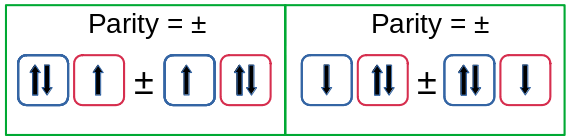
\includegraphics[scale=0.5]{four.png}
\end{center}
\begin{itemize}
\item \(S_z^{tot} = -1\): \(\ket{\uparrow\downarrow,\downarrow}, \ket{\downarrow,\uparrow\downarrow}\)

\beq
\ham \ket{\uparrow\downarrow,\downarrow} = -t \C{2}{\uparrow}\c{1}{\uparrow}\ket{\uparrow\downarrow,\downarrow} + U\ket{\uparrow\downarrow,\downarrow} = -t\ket{\downarrow,\uparrow\downarrow} + U\ket{\uparrow\downarrow,\downarrow} \\
\ham \ket{\downarrow,\uparrow\downarrow} = -t \C{1}{\uparrow}\c{2}{\uparrow}\ket{\downarrow,\uparrow\downarrow} + U\ket{\downarrow,\uparrow\downarrow} = -t\ket{\uparrow\downarrow,\downarrow} + U\ket{\downarrow,\uparrow\downarrow}
\eeq
\beq
\bordermatrix{~ & \ket{\uparrow\downarrow,\downarrow} & \ket{\downarrow,\uparrow\downarrow} \cr
              \ket{\uparrow\downarrow,\downarrow} & U & -t \cr \\
              \ket{\downarrow,\uparrow\downarrow} & -t & U \cr}
\eeq
This matrix has eigenvalues \(U \mp t\), and corresponding eigenvectors \(\frac{\ket{\uparrow\downarrow,\downarrow} \pm \ket{\downarrow,\uparrow\downarrow}}{\sqrt{2}}\)

\item \(S_z^{tot} = +1\): \(\ket{\uparrow\downarrow,\uparrow}, \ket{\uparrow,\uparrow\downarrow}\)

\beq
\ham \ket{\uparrow\downarrow,\uparrow} = -t \C{2}{\downarrow}\c{1}{\downarrow}\ket{\uparrow\downarrow,\uparrow} + U\ket{\uparrow\downarrow,\uparrow} = t \C{2}{\downarrow}\c{1}{\downarrow}\ket{\downarrow\uparrow,\uparrow} + U\ket{\uparrow\downarrow,\uparrow} \\
=t \ket{\uparrow,\downarrow\uparrow} + U\ket{\uparrow\downarrow,\uparrow} = -t \ket{\uparrow,\uparrow\downarrow} + U\ket{\uparrow\downarrow,\uparrow}\\
\ham \ket{\uparrow,\uparrow\downarrow} = -t \C{1}{\downarrow}\c{2}{\downarrow}\ket{\uparrow,\uparrow\downarrow} + U\ket{\uparrow,\uparrow\downarrow} = t \C{1}{\downarrow}\c{2}{\downarrow}\ket{\uparrow,\downarrow\uparrow} + U\ket{\uparrow,\uparrow\downarrow} \\
=t \ket{\downarrow\uparrow,\uparrow} + U\ket{\uparrow,\uparrow\downarrow} = -t \ket{\uparrow\downarrow,\uparrow} + U\ket{\uparrow,\uparrow\downarrow}\\
\eeq

\beq
\bordermatrix{~ & \ket{\uparrow\downarrow,\uparrow} & \ket{\uparrow,\uparrow\downarrow} \cr
              \ket{\uparrow\downarrow,\uparrow} & U & -t \cr \\
              \ket{\uparrow,\uparrow\downarrow} & -t & U \cr}
\eeq
\end{itemize}
This matrix has eigenvalues \(U \mp t\), and corresponding eigenvectors \(\frac{\ket{\uparrow\downarrow,\uparrow} \pm \ket{\uparrow,\uparrow\downarrow}}{\sqrt{2}}\)

\subsection{N = 4}
With four electrons, the only possible state is \(\ket{\uparrow\downarrow,\uparrow\downarrow}\). Its easy to find the eigenvalue. Since all states are filled, no hopping can take place, so the hopping term is zero. Therefore,
\beq
\ham \ket{\uparrow\downarrow,\uparrow\downarrow} = 2U \ket{\uparrow\downarrow,\uparrow\downarrow}
\eeq
So, \(\ket{\uparrow\downarrow,\uparrow\downarrow}\) is an eigenvector with eigenvalue \(2U\).

\subsection{N = 2}

This is the eigenvalue that has the largest subspace.\\\\
\begin{minipage}{\textwidth/2}
\begin{itemize}
\item \(S_z^{tot} = -1\): \(\ket{\downarrow,\downarrow}\)
\item \(S_z^{tot} = +1\): \(\ket{\uparrow,\uparrow}\)
\end{itemize}
\end{minipage}
\begin{minipage}{\textwidth/2}
	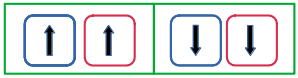
\includegraphics[scale=0.5]{five.png}
\end{minipage}
\vspace*{10pt}\\
These two subspaces have a single state each, so theya are obviously eigenstates. Since they both have identical spins on both sites, the hopping term is 0, and the \(U\)-term is also zero because of single occupation. As a result, they both have zero eigenvalue
\beq
\ham \ket{\downarrow,\downarrow} = \ham \ket{\uparrow,\uparrow} = 0
\eeq
\begin{itemize}
\item \(S_z^{tot} = 0\):  \(\ket{\uparrow,\downarrow},\ket{\downarrow,\uparrow},\ket{0,\uparrow\downarrow},\ket{\uparrow\downarrow,0}\)

This subspace has four eigenvectors,
\beq
\ket{\uparrow,\downarrow},\;\:\;\:\;\:\ket{\downarrow,\uparrow},\;\:\;\:\;\:\ket{0,\uparrow\downarrow},\;\:\;\:\;\:\ket{\uparrow\downarrow,0}
\eeq
so it is not possible to directly diagonalize this subspace. First we organize these states into eigenstates of parity. It is easy by inspection.
\beq
\hat{P}\rr{\ket{\uparrow,\downarrow}\pm\ket{\downarrow,\uparrow}} &= \pm \rr{\ket{\uparrow,\downarrow}\pm\ket{\downarrow,\uparrow}} \\
\hat{P}\rr{\ket{\uparrow\downarrow,0}\pm\ket{0,\uparrow\downarrow}} &= \pm \rr{\ket{\uparrow\downarrow,0}\pm\ket{0,\uparrow\downarrow}}
\eeq
I have the parity eigenstates for this subspace, so its most convenient to work in the basis of these eigenstates
\begin{itemize}
\item \(\hat{P} = 1: \frac{\ket{\uparrow,\downarrow}+\ket{\downarrow,\uparrow}}{\sqrt{2}},\;\:\;\:\;\:\frac{\ket{\uparrow\downarrow,0}+\ket{0,\uparrow\downarrow}}{\sqrt{2}}\)
\item \(\hat{P} = -1: \frac{\ket{\uparrow,\downarrow}-\ket{\downarrow,\uparrow}}{\sqrt{2}},\;\:\;\:\;\:\frac{\ket{\uparrow\downarrow,0}-\ket{0,\uparrow\downarrow}}{\sqrt{2}}\) 
\end{itemize}
Each eigenvalue subspace can now be diagonalized separately. First I look at the eigenstates of \(\hat{P} = 1\). I find the matrix of \(\ham\) in the subspace spanned by these two vectors and then diagonalize that subspace.
\beq
\ham\:\frac{\ket{\uparrow,\downarrow}+\ket{\downarrow,\uparrow}}{\sqrt{2}} &= -\frac{t}{\sqrt{2}} \cc{\rr{\C{1}{\downarrow}\c{2}{\downarrow}+\C{2}{\uparrow}\c{1}{\uparrow}}\ket{\uparrow,\downarrow} +\rr{\C{1}{\uparrow}\c{2}{\uparrow}+\C{2}{\downarrow}\c{1}{\downarrow}}\ket{\downarrow,\uparrow}} \\
&= -\frac{t}{\sqrt{2}}\cc{\ket{\downarrow\uparrow,0}+\ket{0,\uparrow\downarrow}+\ket{\uparrow\downarrow,0}+\ket{0,\downarrow\uparrow}} = 0 \\
\ham\:\frac{\ket{\uparrow\downarrow,0}+\ket{0,\uparrow\downarrow}}{\sqrt{2}} &= -\frac{t}{\sqrt{2}} \cc{\rr{\C{2}{\uparrow}\c{1}{\uparrow}+\C{2}{\downarrow}\c{1}{\downarrow}}\ket{\uparrow\downarrow,0} + \rr{\C{1}{\uparrow}\c{2}{\uparrow}+\C{1}{\downarrow}\c{2}{\downarrow}}\ket{0,\uparrow\downarrow}} +U\frac{\ket{\uparrow\downarrow,0}+\ket{0,\uparrow\downarrow}}{\sqrt{2}} \\
&= -\frac{t}{\sqrt{2}}\cc{\ket{\downarrow,\uparrow}-\ket{\uparrow,\downarrow}+\ket{\uparrow,\downarrow}-\ket{\downarrow,\uparrow}} +U\frac{\ket{\uparrow\downarrow,0}+\ket{0,\uparrow\downarrow}}{\sqrt{2}} = U\frac{\ket{\uparrow\downarrow,0}+\ket{0,\uparrow\downarrow}}{\sqrt{2}}
\eeq
We get the following matrix
\beq
\bordermatrix{~ & \frac{\ket{\uparrow,\downarrow}+\ket{\downarrow,\uparrow}}{\sqrt{2}} & \frac{\ket{\uparrow\downarrow,0}+\ket{0,\uparrow\downarrow}}{\sqrt{2}} \cr
              \frac{\ket{\uparrow,\downarrow}+\ket{\downarrow,\uparrow}}{\sqrt{2}} & 0 & 0 \cr \\
              \frac{\ket{\uparrow\downarrow,0}+\ket{0,\uparrow\downarrow}}{\sqrt{2}} & 0 & U \cr}
\eeq
As it appears, the subspace is already diagonal in the eigenbasis of \(\hat{P}\). The \(\hat{P} = 1\) eigenstates are eigenstates of \(\ham\), with eigenvalues 0 and \(U\). Next I look at the eigenstates of \(\hat{P}=-1\).

\beq
\ham\:\frac{\ket{\uparrow,\downarrow}-\ket{\downarrow,\uparrow}}{\sqrt{2}} &= -\frac{t}{\sqrt{2}} \cc{\rr{\C{1}{\downarrow}\c{2}{\downarrow}\C{2}{\uparrow}\c{1}{\uparrow}}\ket{\uparrow,\downarrow} -\rr{\C{1}{\uparrow}\c{2}{\uparrow}+\C{2}{\downarrow}\c{1}{\downarrow}}\ket{\downarrow,\uparrow}} \\
&= -\frac{t}{\sqrt{2}}\cc{\ket{\downarrow\uparrow,0}+\ket{0,\uparrow\downarrow}-\ket{\uparrow\downarrow,0}-\ket{0,\downarrow\uparrow}} \\
&= 2t\frac{\ket{\uparrow\downarrow,0}-\ket{0,\uparrow\downarrow}}{\sqrt{2}} \\
\ham\:\frac{\ket{\uparrow\downarrow,0}-\ket{0,\uparrow\downarrow}}{\sqrt{2}} &= -\frac{t}{\sqrt{2}} \cc{\rr{\C{2}{\uparrow}\c{1}{\uparrow}+\C{2}{\downarrow}\c{1}{\downarrow}}\ket{\uparrow\downarrow,0} - \rr{\C{1}{\uparrow}\c{2}{\uparrow}+\C{1}{\downarrow}\c{2}{\downarrow}}\ket{0,\uparrow\downarrow}} +U\frac{\ket{\uparrow\downarrow,0}+\ket{0,\uparrow\downarrow}}{\sqrt{2}} \\
&= -\frac{t}{\sqrt{2}}\cc{\ket{\downarrow,\uparrow}-\ket{\uparrow,\downarrow}-\ket{\uparrow,\downarrow}+\ket{\downarrow,\uparrow}} +U\frac{\ket{\uparrow\downarrow,0}+\ket{0,\uparrow\downarrow}}{\sqrt{2}} \\
&= 2t\frac{\ket{\uparrow,\downarrow}-\ket{\downarrow,\uparrow}}{2} + U\frac{\ket{\uparrow\downarrow,0}-\ket{0,\uparrow\downarrow}}{\sqrt{2}}
\eeq
\beq
\bordermatrix{~ & \frac{\ket{\uparrow,\downarrow}-\ket{\downarrow,\uparrow}}{\sqrt{2}} & \frac{\ket{\uparrow\downarrow,0}-\ket{0,\uparrow\downarrow}}{\sqrt{2}} \cr
              \frac{\ket{\uparrow,\downarrow}-\ket{\downarrow,\uparrow}}{\sqrt{2}} & 0 & 2t \cr \\
              \frac{\ket{\uparrow\downarrow,0}-\ket{0,\uparrow\downarrow}}{\sqrt{2}} & 2t & U \cr}
\eeq
This subspace is not automatically diagonal, but is easily diagonalized. The eigenvectors are 
\beq
&\frac{1}{N_\pm}\cc{2t \frac{(\ket{\uparrow,\downarrow}-\ket{\downarrow,\uparrow})}{\sqrt{2}} + \frac{U\pm\sqrt{U^2+16 t^2}}{2} \frac{(\ket{\uparrow\downarrow,0}-\ket{0,\uparrow\downarrow})}{\sqrt{2}}} \\
&N_{\pm} = \cc{\frac{U}{2}\qq{U\pm\sqrt{U^2+16t^2}}+16t^2}^\frac{1}{2}
\eeq
with eigenvalues \(\frac{U\pm\sqrt{U^2+16 t^2}}{2}\) respectively.
\end{itemize}

\begin{center}
	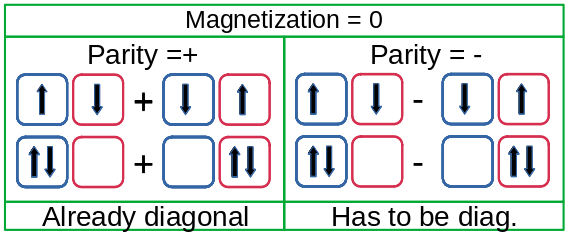
\includegraphics[scale=0.5]{six.png}
\end{center}


\subsection{The total spectrum}
\begin{center}
\begin{tabular}{@{}ccccc@{}}
\toprule
	\multicolumn{5}{c}{\bf{Exact diagonalization of Hubbard dimer (real space)}} \\
\toprule
\(\hat{N}\) & \(S_z^{tot}\) & \(\hat{P}\) & E & \(\ket{\Phi}\)\\
\toprule
0 & - & - & 0 & \(\ket{0,0}\) \\ \toprule
\multicolumn{1}{c}{\multirow{4}{*}{1}} & \multirow{2}{*}{-1} & 1  & -t  & \(\frac{\ket{\downarrow,0}+\ket{0,\downarrow}}{\sqrt{2}}\)  \\ \cmidrule(l){3-5} 
\multicolumn{1}{c}{}                   &                     & -1 & t   & \(\frac{\ket{\downarrow,0}-\ket{0,\downarrow}}{\sqrt{2}}\)  \\ \cmidrule(l){2-5}
\multicolumn{1}{c}{}                   & \multirow{2}{*}{1}  & 1  & -t  & \(\frac{\ket{\uparrow,0}+\ket{0,\uparrow}}{\sqrt{2}}\)  \\ \cmidrule(l){3-5} 
\multicolumn{1}{c}{}                   &                     & -1 & t   & \(\frac{\ket{\uparrow,0}-\ket{0,\uparrow}}{\sqrt{2}}\)  \\ \toprule
\multirow{6}{*}{2}                     & -1                  & 1  & 0   & \(\ket{\downarrow,\downarrow}\)  \\ \cmidrule(l){2-5} 
                                       & \multirow{4}{*}{0}  & 1  & 0   & \(\frac{\ket{\uparrow,\downarrow}+\ket{\downarrow,\uparrow}}{\sqrt{2}}\)  \\ \cmidrule(l){3-5} 
                                       &                     & 1  & U   & \(\frac{\ket{\uparrow\downarrow,0}+\ket{0,\uparrow\downarrow}}{\sqrt{2}}\)  \\ \cmidrule(l){3-5} 
                                       &                     & -1 & \(\frac{U+\sqrt{U^2+16 t^2}}{2}\)    & \(\frac{1}{N_+}\cc{2t \frac{(\ket{\uparrow,\downarrow}-\ket{\downarrow,\uparrow})}{\sqrt{2}} + \frac{U+\sqrt{U^2+16 t^2}}{2} \frac{(\ket{\uparrow\downarrow,0}-\ket{0,\uparrow\downarrow})}{\sqrt{2}}}\)  \\ \cmidrule(l){3-5} 
                                       &                     & -1 & \(\frac{U-\sqrt{U^2+16 t^2}}{2}\)    & \(\frac{1}{N_-}\cc{2t \frac{(\ket{\uparrow,\downarrow}-\ket{\downarrow,\uparrow})}{\sqrt{2}} + \frac{U-\sqrt{U^2+16 t^2}}{2} \frac{(\ket{\uparrow\downarrow,0}-\ket{0,\uparrow\downarrow})}{\sqrt{2}}}\)  \\ \cmidrule(l){2-5} 
                                       & 1                   & 1  & 0   & \(\ket{\uparrow,\uparrow}\) \\ \toprule
\multirow{4}{*}{3}                     & \multirow{2}{*}{-1} & 1  & U-t & \(\frac{\ket{\uparrow\downarrow,\downarrow}+\ket{\downarrow,\uparrow\downarrow}}{\sqrt{2}}\) \\ \cmidrule(l){3-5} 
                                       &                     & -1 & U+t & \(\frac{\ket{\uparrow\downarrow,\downarrow}-\ket{\downarrow,\uparrow\downarrow}}{\sqrt{2}}\) \\ \cmidrule(l){2-5}
                                       & \multirow{2}{*}{1}  & 1  & U-t & \(\frac{\ket{\uparrow\downarrow,\uparrow}+\ket{\uparrow,\uparrow\downarrow}}{\sqrt{2}}\) \\ \cmidrule(l){3-5} 
                                       &                     & -1 & U+t & \(\frac{\ket{\uparrow\downarrow,\uparrow}-\ket{\uparrow,\uparrow\downarrow}}{\sqrt{2}}\) \\ \toprule
4                                      & 0                   & 1  & 2U  & \(\ket{\uparrow\downarrow,\uparrow\downarrow}\) \\
\toprule
\end{tabular}
\end{center}
\subsection{The Mott-insulating limit}
In the limit of \il{U\gg t}, the \il{N=2} part of the spectrum groups itself roughly into two bands:
\begin{gather}
\fr{U+\sqrt{U^2+16t^2}}{2} =  \fr{U+U\sqrt{1+\fr{16t^2}{U}}}{2} \approx \fr{U+U(1+\fr{8t^2}{U^2})}{2} = U + \fr{4t^2}{U}\\
\fr{U-\sqrt{U^2+16t^2}}{2} =  \fr{U-U\sqrt{1+\fr{16t^2}{U}}}{2} \approx \fr{U-U(1+\fr{8t^2}{U^2})}{2} = -\fr{4t^2}{U}
\end{gather}
\begin{center}
\begin{tabular}{|c|c|c|}
    \hline
    \multirow{2}{*}{lower} & \il{\fr{-4t^2}{U}} & \il{\fr{\ket{\ua,\da}-\ket{\da,\ua}}{\sqrt 2}} \\
    & \il{0} & \il{\ket{\ua,\ua}, \ket{\da,\da}, \fr{\ket{\ua,\da}+\ket{\da,\ua}}{\sqrt 2}}\\
    \hline
    \multirow{2}{*}{upper} & \il{U} & \il{\fr{\ket{\ua\da,0}+\ket{0,\ua\da}}{\sqrt 2}} \\
    & \il{U+\fr{4t^2}{U}} & \il{\fr{\ket{\ua\da,0}-\ket{0,\ua\da}}{\sqrt 2}}\\
    \hline
\end{tabular}
\end{center}
\begin{itemize}
    \item The separation between the two bands is \il{\Delta=U}. The kets in the lower band are formed mostly  of superpositions of the Neel states (singly occupied states with opposite spin) as well as the polarised states (singly occupied states with same spin). This is expected because for very large \il{U}, it becomes the only determining factor, and states with single occupation will be appreciably lower in energy compared to the doubly occupied states, and hence will gather in the lower band. 
    \item For exactly the same reason, the upper band will be formed mostly by superpositions of holon-doublon states (two electrons on one site and none on the other), because they will incur the heavy cost of the on-site repulsion energy, and will hence assemble in the upper band. 
    \item The lower band is a collection of three states: the ground state is the singlet state \il{\ket{\ua,\da}-\ket{\da,\ua}}, with an energy of \il{-\fr{4t^2}{U}}, while the other three , \il{\ket{\ua,\ua},\ket{\da,\da}, \ket{\ua,\da}+\ket{\da,\ua}}, form a degenerate triplet of first excited states with \il{0} energy.
\end{itemize}
\subsection{Comparison with the antiferromagnetic Heisenberg model}
\beq
\ham_{\text{Heisenberg}} = J \vec{\sigma_1}\cdot\vec{\sigma_2} - J, && \text{with  }J=-\fr{t^2}{U}<0
\eeq
To diagonalise this Hamiltonian, we rewrite the pauli matrix vectors using \il{\sigma^z} and \il{\sigma^\pm}:
\beq
\vec{\sigma_1}\cdot\vec{\sigma_2} = \sigma^z_1\sigma^z_2 + \fr{\sigma^+_1\sigma^-_2+\sigma^-_1\sigma^+_2}{2}
\eeq
where \il{\sigma^\pm_i = \sigma^x_i \pm \iota\sigma^y_i}. Note that 
\begin{gather}
    \sigma^+\ket{\ua}=\sigma^-\ket{\da} = 0\\
    \sigma^+\ket{\da}=2\ket{\ua}\\
    \sigma^-\ket{\ua}=2\ket{\da}
\end{gather}
Using these properties, it is easy to write down the \il{4\times4} matrix of the Hamiltonian in the basis of \il{\ket{\ua\ua},\ket{\ua\da},\ket{\da\ua},\ket{\da\da}}.
\beq
\ham = J \begin{pmatrix}
    1 & & & \\
    & -1 & 2 & \\
    & 2 & -1 & \\
    & & & 1 \\
\end{pmatrix}
- J
\eeq

The \il{\ket{\ua\ua}} and \il{\ket{\da\da}} form eigenkets with eigenvalues J each. The middle \il{2\times2} matrix can easily be diagonalised. It gives two other eigenvectors \il{\ket{\ua\da}\pm\ket{\da\ua}}, with eigenvalues \il{J,-3J}. After adding the constant term \il{-J} to these eigenvalues, the final spectrum becomes
\begin{itemize}
    \item \il{\ket{\ua\ua}: 0}
    \item \il{\ket{\da\da}: 0}
    \item \il{\ket{\ua\da}+\ket{\da\ua}: 0}
    \item \il{\ket{\ua\da}-\ket{\da\ua}: -4J}
\end{itemize}
Recognizing \il{J} as \il{-\fr{t^2}{U}}, we get the same spectrum as the lower block.

\subsection{Diagonalization in momentum space}
Since I will also need the momentum space eigenvectors later, I am briefly showing the process here. The process is simpler compared to the real space process, because of the translational invariance. It is similarly possible to diagonalise the momentum space Hamiltonian. To write the Hamiltonian in momentum space, note that the allowed values of the momentum are \il{k_n = n\pi = 0,\pi}. Using these modes, the creation and annihilation operators can be Fourier transformed:
\beq
c_{1,\sigma}=\fr{1}{\sqrt 2}\rr{c_{0,\sigma}+c_{\pi,\sigma}}\\
c_{2,\sigma}=\fr{1}{\sqrt 2}\rr{c_{0,\sigma}-c_{\pi,\sigma}}
\eeq
In terms of these operators, the Hubbard Hamiltonian becomes
\beq
\ham = t\rr{\hat n_{\pi}-\hat n_{0}}+\fr{U}{2}n_\ua n_\da + \fr{U}{2}\prod_\sigma \qq{c^\dagger_{0,\sigma}c_{\pi,\sigma}+c^\dagger_{\pi,\sigma}c_{0,\sigma}}
\eeq
\begin{minipage}{300pt}
where \il{n_\pi = \sum_\sigma n_{\pi\sigma}}. This Hamiltonian also conserves the total particle number and z-component of total spin. The notation used is \il{\ket{n_{\pi\ua}n_{\pi\da},n_{0\ua}n_{0\da}}}.
\end{minipage}
\hspace{10pt}
\begin{minipage}{\textwidth/3}
	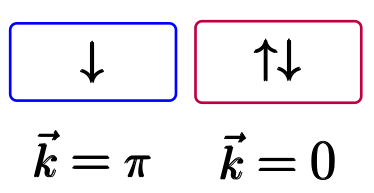
\includegraphics[scale=0.3]{pic3.png}
\end{minipage}

\paragraph{N=1}

\beq
\ham \ket{\ua,0} &= t \ket{\ua,0}\\ 
\ham \ket{\da,0} &= t \ket{\da,0}\\ 
\ham \ket{0,\ua} &= -t\ket{0,\ua}\\ 
\ham \ket{0,\da} &= -t\ket{0,\da}\\ 
\eeq

\paragraph{N=2}

\beq
\ham \ket{\ua,\ua} &= 0\ket{\ua,\ua}\\
\ham \ket{\da,\da} &= 0\ket{\da,\da}\\
\ham \ket{\ua,\da} &= \fr{U}{2}\ket{\ua,\da} - \fr{U}{2}\ket{\da,\ua}\\
\ham \ket{\da,\ua} &= \fr{U}{2}\ket{\da,\ua} - \fr{U}{2}\ket{\ua,\da}\\
\fr{U}{2}\begin{pmatrix} 1 & -1 \\ -1 & 1 \end{pmatrix} &\implies 0,U \implies \ket{\ua,\da}\pm\ket{\da,\ua}\\
\ham \ket{\ua\da,0} &= (2t + \fr{U}{2})\ket{\ua\da,0} - \fr{U}{2}\ket{0,\ua\da}\\
\ham \ket{0,\ua\da} &= (-2t + \fr{U}{2})\ket{0,\ua\da} - \fr{U}{2}\ket{\ua\da,0}\\
\fr{U}{2}+\begin{pmatrix} 2t & -\fr{U}{2} \\ -\fr{U}{2} & -2t \end{pmatrix} &\implies \fr{U\pm\Delta}{2} \implies \fr{U}{2}\ket{\ua\da,0}+(2t\pm\Delta)\ket{0,\ua\da}
\eeq

\paragraph{N = 3}

\beq
\ham \ket{\ua,\ua\da} &= (-t+U) \ket{\ua,\ua\da}\\ 
\ham \ket{\da,\ua\da} &= (-t+U) \ket{\da,\ua\da}\\ 
\ham \ket{\ua\da,\ua} &= (t +U) \ket{\ua\da,\ua}\\ 
\ham \ket{\ua\da,\da} &= (t +U) \ket{\ua\da,\da}\\ 
\eeq

\newpage
\section{Exact diagonalization of the Anderson molecule}
\pp[The Hamiltonian]
\beq
\ham = -t\sum_\sigma\rr{\C{1}{\sigma}\c{2}{\sigma}+\C{2}{\sigma}\c{1}{\sigma}} + U\hat{n}_{1\uparrow}\hat{n}_{1\downarrow} + \epsilon_s\sum_\sigma\hat n_{2\sigma} + \epsilon_d\sum_\sigma\hat n_{1\sigma}
\eeq

This is quite similar to the Hubbard dimer Hamiltonian. The difference here is that the first site represents an impurity site with energy \il{\epsilon_d}, and the second site represents the conduction band with chemical potential \il{\epsilon_s}. The single particle energy levels are \il{epsilon_d} if the site is unoccupied and \il{\epsilon_d+U} if one electron is already there. For simplicity, I will set the chemical potential to exactly midway between these two levels : \il{\epsilon_d+\fr{U}{2}}.

\subsection{Symmetries of the problem}
The following operators commute with the Hamiltonian.
\begin{enumerate}
\item\bf{Total number operator}: \(\qq{\ham, \hat N}=0\).
\item \bf{Magnetization operator}: \(\qq{\ham, \hat{S}^z_{tot}}=0\).
\item \bf{Total Spin Operator}: Total spin angular momentum operator,
\beq
\hat S^2_{tot} = \hat (S^x_{tot})^2 + \hat (S^y_{tot})^2 + \hat (S^z_{tot})^2 = S_{tot}^+S_{tot}^- - \hbar S_{tot}^z + (S_{tot}^z)^2
\eeq
Since all the terms in the Hamiltonian are spin-preserving (all events conserve the number of particles having a definite spin \(\sigma\)), total angular momentum will be conserved. It's obvious that the number operator term do so. The hopping term does so as well; \(c^\dagger_{i\sigma}c_{j\sigma}\) destroys a particle of spin \(\sigma\) and creates a particle of the same spin; the total angular momentum remain conserved in the process, although the number of particles at a particular site is not conserved. Thus, \(\qq{\hat S^2_{tot}, \ham}=0\).
\end{enumerate}

\subsection{N = 1 sector}
\begin{itemize}
\item \(S_{tot}^z = -1\): \(\ket{\downarrow,0}, \ket{0, \downarrow}\)

\beq
\ham\ket{\downarrow,0} = \epsilon_d\ket{\downarrow,0}-t\ket{0,\downarrow} \\
\ham\ket{0,\downarrow} = \epsilon_s\ket{0,\downarrow}-t\ket{\downarrow,0} \\
\eeq
We get the following matrix for this tiny subspace of the Hamiltonian:
\beq
\bordermatrix{~ & \ket{\downarrow,0} & \ket{0,\downarrow} \cr
              \ket{\downarrow,0} & \epsilon_d\ & -t \cr \\
              \ket{0,\downarrow} & -t & \epsilon_s \cr}
\eeq
Eigenvalues: \(\fr{1}{2}\qq{\epsilon_d+\epsilon_s \pm \sqrt{(\epsilon_d-\epsilon_s)^2+4t^2}}\). For \(\epsilon_s = \epsilon_d + \fr{U}{2}\) and \(\Delta = \sqrt{U^2+16t^2}\), \\ eigenvalues, \(\lambda_\pm = \epsilon_d + \fr{1}{4}(U\pm\Delta)\). \\
The eigenvectors are \(\fr{1}{N_\pm}\rr{t\ket{\downarrow,0}-\fr{1}{4}(U\pm\Delta)\ket{0,\downarrow}}\), where \(N_\pm^2 = t^2 + (\fr{U\pm\Delta}{4})^2\)


\item \(S_{tot}^z = +1\): \(\ket{\uparrow,0}, \ket{0, \uparrow}\)
\end{itemize}

\beq
\ham\ket{\uparrow,0} = \epsilon_d\ket{\uparrow,0}-t\ket{0,\uparrow} \\
\ham\ket{0,\uparrow} = \epsilon_s\ket{0,\uparrow}-t\ket{\uparrow,0} \\
\eeq
Clearly, this gives the same matrix as the spin-down states. So, the eigenvalues will be exactly the same, and the eigenvectors will be correspondingly modified in the new basis. \\
eigenvectors : \(\fr{1}{N_\pm}\rr{t\ket{\uparrow,0}+(\epsilon_d-\lambda_\pm)\ket{0,\uparrow}}\)
\subsection{N = 3 sector}
\begin{itemize}
\item \(S_{tot}^z = -1\): \(\ket{\uparrow\downarrow,\downarrow}, \ket{\downarrow,\uparrow\downarrow}\)

\beq
\ham \ket{\uparrow\downarrow,\downarrow} = -t\ket{\downarrow,\uparrow\downarrow} + (2\epsilon_d + \epsilon_s + U)\ket{\uparrow\downarrow,\downarrow} \\
\ham \ket{\downarrow,\uparrow\downarrow} = -t\ket{\uparrow\downarrow,\downarrow} + (2\epsilon_s + \epsilon_d)\ket{\downarrow,\uparrow\downarrow}
\eeq
\beq
\bordermatrix{~ & \ket{\uparrow\downarrow,\downarrow} & \ket{\downarrow,\uparrow\downarrow} \cr
              \ket{\uparrow\downarrow,\downarrow} & 2\epsilon_d + \epsilon_s + U & -t \cr \\
              \ket{\downarrow,\uparrow\downarrow} & -t & 2\epsilon_s + \epsilon_d \cr}
\eeq
Again setting \(\epsilon_s = \epsilon_d + \fr{U}{2}\), eigenvalues: \(3\epsilon_d + \fr{5}{4}U \pm \fr{1}{4}\Delta\). \\ Corresponding eigenvectors \(\fr{1}{N_\pm}(t\ket{\uparrow\downarrow,\downarrow}+\fr{1}{4}(U\mp\Delta)\ket{\downarrow,\uparrow\downarrow})\)

\item \(S_{tot}^z = +1\): \(\ket{\uparrow\downarrow,\uparrow}, \ket{\uparrow,\uparrow\downarrow}\)
\end{itemize}

\beq
\ham \ket{\uparrow\downarrow,\uparrow} = -t\ket{\uparrow,\uparrow\downarrow} + (2\epsilon_d + \epsilon_s + U)\ket{\uparrow\downarrow,\uparrow} \\
\ham \ket{\uparrow,\uparrow\downarrow} = -t\ket{\uparrow\downarrow,\uparrow} + (2\epsilon_s + \epsilon_d)\ket{\uparrow,\uparrow\downarrow}
\eeq
Again the same matrix. Hence the eigenvalues are same. Eigenvectors are
\(\fr{1}{N_\pm}(t\ket{\uparrow\downarrow,\uparrow}-\fr{1}{4}(U\pm\Delta)\ket{\uparrow,\uparrow\downarrow})\)

\subsection{N = 2 sector}

This is the eigenvalue that has the largest subspace.

\begin{itemize}
\item \(S_{tot}^z = -1\): \(\ket{\downarrow,\downarrow}\)
\item \(S_{tot}^z = +1\): \(\ket{\uparrow,\uparrow}\)

These two subspaces have a single state each, so theya are obviously eigenstates. Since they both have identical spins on both sites, the hopping term is 0, and the \(U\)-term is also zero because of single occupation. As a result, they both have zero eigenvalue
\beq
\ham \ket{\downarrow,\downarrow} = \ham \ket{\uparrow,\uparrow} = \epsilon_s + \epsilon_d
\eeq

\item \(S_{tot}^z = 0\):  \(\ket{\uparrow,\downarrow},\ket{\downarrow,\uparrow},\ket{0,\uparrow\downarrow},\ket{\uparrow\downarrow,0}\)
\end{itemize}

This subspace has four eigenvectors,
\beq
\ket{\uparrow,\downarrow},\;\:\;\:\;\:\ket{\downarrow,\uparrow},\;\:\;\:\;\:\ket{0,\uparrow\downarrow},\;\:\;\:\;\:\ket{\uparrow\downarrow,0}
\eeq
so it is easier to first find eigenstates of \(S^2_{tot}\). Since these are states with zero \(S^z\), \(S^2_{tot}\) for these states is just \(S^+S^-\)
\beq
&S^+S^-\ket{\uparrow,\downarrow} = S^+S^-\ket{\downarrow,\uparrow} = \ket{\uparrow,\downarrow} + \ket{\downarrow,\uparrow} \\
&S^+S^-\ket{\uparrow\downarrow,0} = S^+S^-\ket{0,\uparrow\downarrow} = 0 \\
\eeq
The eigenstates are
\beq
\fr{\ket{\uparrow,\downarrow} + \ket{\downarrow,\uparrow}}{\sqrt 2} (S^2_{tot}=1), \;\;\;\;\cc{\fr{\ket{\uparrow,\downarrow} - \ket{\downarrow,\uparrow}}{\sqrt 2}, \ket{\uparrow\downarrow,0}, \ket{0,\uparrow\downarrow}} (S^2_{tot}=0) \\
\eeq
\(S^2_{tot}=1\) immediately delivers an eigenstate:
\beq
\ham\fr{\ket{\uparrow,\downarrow} + \ket{\downarrow,\uparrow}}{\sqrt 2} = (\epsilon_d+\epsilon_s)\rr{\fr{\ket{\uparrow,\downarrow} + \ket{\downarrow,\uparrow}}{\sqrt 2}}
\eeq
Next I diagonalize the subspace \(S^2_{tot}=0\). 
\beq
\ham\fr{\ket{\uparrow,\downarrow} - \ket{\downarrow,\uparrow}}{\sqrt 2} &= (\epsilon_d+\epsilon_s)\rr{\fr{\ket{\uparrow,\downarrow} - \ket{\downarrow,\uparrow}}{\sqrt 2}} + \sqrt{2}t(\ket{\uparrow\downarrow,0} - \ket{0,\uparrow\downarrow}) \\
\ham\ket{\uparrow\downarrow,0} &= (2\epsilon_d+U)\ket{\uparrow\downarrow,0} + \sqrt{2}t\fr{\ket{\uparrow,\downarrow} - \ket{\downarrow,\uparrow}}{\sqrt 2} \\
\ham\ket{0,\uparrow\downarrow} &= (2\epsilon_d+U)\ket{0,\uparrow\downarrow} - \sqrt{2}t\fr{\ket{\uparrow,\downarrow} - \ket{\downarrow,\uparrow}}{\sqrt 2}
\eeq
We get the following matrix
\beq
\begin{pmatrix}
	2\epsilon_d+\fr{U}{2} & \sqrt{2}t & -\sqrt{2}t \\
	\sqrt{2}t & 2\epsilon_d+U & 0 \\
	-\sqrt{2}t & 0 & 2\epsilon_d+U
\end{pmatrix}
\eeq
The eigenvectors are
\begin{itemize}
	\item \(\ket{\uparrow\downarrow,0} - \ket{0,\uparrow\downarrow}: 2\epsilon_d+U\)
	\item \(\fr{U-\Delta}{4\sqrt{2}t}\fr{\ket{\uparrow,\downarrow} - \ket{\downarrow,\uparrow}}{\sqrt 2}-\ket{\uparrow\downarrow,0} + \ket{0,\uparrow\downarrow}: 2\epsilon_d+\fr{3}{4}U+\fr{1}{2}\Delta(\fr{U}{2},t)\)
	\item \(\fr{U+\Delta}{4\sqrt{2}t}\fr{\ket{\uparrow,\downarrow} - \ket{\downarrow,\uparrow}}{\sqrt 2}-\ket{\uparrow\downarrow,0} + \ket{0,\uparrow\downarrow}: 2\epsilon_d+\fr{3}{4}U-\fr{1}{2}\Delta(\fr{U}{2},t)\)
\end{itemize}

\subsection{The total spectrum}

\begin{center}
\begin{tabular}{@{}cccc@{}}
\toprule
\multicolumn{4}{c}{\bf{Exact Diagonalization of Anderson Molecule}} \\
\toprule
\(\hat{N}\) & \(S_{tot}^z\) & E & \(\ket{\Phi}\)\\
\toprule
0 & - & 0 & \(\ket{0,0}\) \\ \toprule
\multirow{2}{*}{1} & -1 & \(\epsilon_d + \fr{1}{4}(U\pm\Delta)\)  & \(\fr{1}{N_\pm}\rr{t\ket{\downarrow,0}-\fr{1}{4}(U\pm\Delta)\ket{0,\downarrow}}\) \\

 \cmidrule(l){2-4}

& 1 & \(\epsilon_d + \fr{1}{4}(U\pm\Delta)\)  & \(\fr{1}{N_\pm}\rr{t\ket{\ua,0}-\fr{1}{4}(U\pm\Delta)\ket{0,\ua}}\) \\
 \toprule

\multirow{6}{*}{2}                     & -1                  & \(2\epsilon_d+\fr{U}{2}\)   & \(\ket{\downarrow,\downarrow}\)  \\
 \cmidrule(l){2-4} 
                                       & 1                   & \(2\epsilon_d+\fr{U}{2}\)   & \(\ket{\uparrow,\uparrow}\) \\
                                       \cmidrule(l){2-4} 
                                       & \multirow{3}{*}{0}  & \(2\epsilon_d+\fr{U}{2}\)   & \(\frac{\ket{\uparrow,\downarrow}+\ket{\downarrow,\uparrow}}{\sqrt{2}}\)  \\
                                        \cmidrule(l){3-4} 

                                       &                     & \(2\epsilon_d+U\)  & \(\frac{\ket{\uparrow\downarrow,0}+\ket{0,\uparrow\downarrow}}{\sqrt{2}}\)  \\
                                        \cmidrule(l){3-4} 

                                       &                     & \(2\epsilon_d+\fr{3}{4}U\pm\fr{1}{2}\Delta(\fr{U}{2},t)\)    & \(\fr{U\mp\Delta}{4\sqrt{2}t}\fr{\ket{\uparrow,\downarrow} - \ket{\downarrow,\uparrow}}{\sqrt 2}-\ket{\uparrow\downarrow,0} + \ket{0,\uparrow\downarrow}\)  \\
                                     
                                        \toprule

\multirow{2}{*}{3} & -1 & \(3\epsilon_d + \fr{5}{4}U \pm \fr{1}{4}\Delta\)  & \(\fr{1}{N_\pm}(t\ket{\uparrow\downarrow,\downarrow}+\fr{1}{4}(U\mp\Delta)\ket{\downarrow,\uparrow\downarrow})\) \\

 \cmidrule(l){2-4}

& 1 & \(3\epsilon_d + \fr{5}{4}U \pm \fr{1}{4}\Delta\)  & \(\fr{1}{N_\pm}(t\ket{\uparrow\downarrow,\uparrow}+\fr{1}{4}(U\mp\Delta)\ket{\uparrow,\uparrow\downarrow})\) \\
 \toprule

4                                      & 0                   & 2(\(\epsilon_s+\epsilon_d)+U\)  & \(\ket{\uparrow\downarrow,\uparrow\downarrow}\) \\
\toprule
\end{tabular}
\end{center}

\subsection{The Kondo molecule limit}
In the limit of large \il{U}, the Anderson molecule in the \il{N=2} sector effectively develops an antiferromagnetic interaction, and the spectrum splits into two bands. This is similar to the case of Hubbard dimer, where the spectrum matched that of an antiferromagnetic Heisenberg system at large U. The difference is in the value of the Heisenberg parameter \il{J}.

First set \il{\epsilon_d = -\frac{U}{2}} to impose particle-hole symmetry (the impurity part of the Hamiltonian then becomes invariant under changing the particle operators to hole operators). In the limit of large \il{U},
\begin{gather}
	\Delta\rr{\fr{U}{2}, t} = \sqrt{\fr{U^2}{4}+16t^2} \approx \fr{U}{2} + \fr{16t^2}{U}
\end{gather}
\begin{center}
\begin{tabular}{|c|c|c|c|}
	\hline
	before & after & states & band \\
    \hline
	\(2\epsilon_d+\fr{3}{4}U-\fr{1}{2}\Delta(\fr{U}{2},t)\)& \il{\fr{-8t^2}{U}} & \il{\fr{\ket{\ua,\da}-\ket{\da,\ua}}{\sqrt 2}} & \multirow{2}{*}{lower}  \\
	\il{2\epsilon_d+\fr{U}{2}} & \il{0} & \il{\ket{\ua,\ua}, \ket{\da,\da}, \fr{\ket{\ua,\da}+\ket{\da,\ua}}{\sqrt 2}} & \\
    \hline
	\il{2\epsilon_d+U} & \il{\fr{U}{2}} & \il{\fr{\ket{\ua\da,0}+\ket{0,\ua\da}}{\sqrt 2}} & \multirow{2}{*}{upper}  \\
	\(2\epsilon_d+\fr{3}{4}U+\fr{1}{2}\Delta(\fr{U}{2},t)\)& \il{\fr{U}{2}+\fr{8t^2}{U}} & \il{\fr{\ket{\ua\da,0}-\ket{0,\ua\da}}{\sqrt 2}}&\\
    \hline
\end{tabular}
\end{center}


\newpage

\section{Block-diagonalization of a Fermionic Hamiltonian}

\subsection{The Problem}
I have a system of \(N\) spin-half fermions. The corresponding Hamiltonian \(\hml\) comprises \(2N\) fermionic single particle degrees of freedom defined in the number occupancy basis of \(\hat{n}_{i\sigma} = c^\dagger_{i\sigma}c_{i\sigma}\), for all \([i\sigma]\in[1,N]\times[\sigma,-\sigma]\). The corresponding Hilbert space has a dimension of \(2^{2N}\). \(i\) represents some external degree of freedom like site-index for electrons on a lattice or the electron momentum if we go to momentum-space. This Hamiltonian is in general non-diagonal in the occupancy basis of a certain degree of freedom \(N\sigma\). \(N\sigma\) can be taken to be any degree of freedom, like say, the first lattice site or the largest momentum (Fermi momentum for a Fermi gas). Equivalently, for a general \ham, \(\qq{\ham, \hat{n}_{N\sigma}}\neq 0\). The goal is to diagonalize this Hamiltonian. 

\subsection{Writing the Hamiltonian as blocks}
The Hamiltonian \(\hml\) in general has off-diagonal terms and can be written as the following general matrix in the occupancy basis of \(N\sigma\):
\beq
\hml = \bordermatrix{~ & \ket{1} & \ket{0} \cr
              \bra{1} & H_1 & H_2 \cr \\
              \bra{0} & H_3 & H_4 \cr}
\eeq
where \(\ket{1} \equiv \ket{\no=1}\) (occupied). Note that the \(H_i\) are not scalars but matrices(blocks), of dimension half that of \(\hml\), that is \(2^{2N-1}\). Its clear that since, for example, \(H_2 = \bra{1}\hml\ket{0}\), we have
\beq[ham-martix]
\hml = H_1 \no + c_{N\sigma}^\dagger H_2 + H_3 c_{N\sigma} +H_4(1-\no)
\eeq
Its trivial to check that this definition of \(\hml\) indeed gives back the mentioned matrix elements. The expression for these matrix elements is quite easy to calculate. First, we define the partial trace over the subspace \(N\sigma\)
\beq
Tr_{N\sigma} \rr{\hml} \equiv \sum_{\ket{N\sigma}}\bra{N\sigma}\hml\ket{N\sigma} 
\eeq
The sum is over the possible states of \(N\sigma\), that is, \(\no=0\) and \(\no=1\). Applying this partial trace to equation \ref{ham-martix}, after multiplying throughout with \(\no\) from the right, gives
\beq
Tr_{N\sigma} \rr{\hml\no} = Tr_{N\sigma} \qq{H_1 \no \no + c_{N\sigma}^\dagger H_2\no + H_3 c_{N\sigma}\no +H_4(1-\no)\no}
\eeq
Recall the following: \(\no^2=\no\), \((1-\no)\no=0\). \\\\
Also, since \(H_i\) are matrix elements with respect to \no, they will commute with the creation and annihilation operators. Hence, \(Tr_{N\sigma}(c_{N\sigma}^\dagger H_2\no) = H_2 Tr_{N\sigma}(c_{N\sigma}^\dagger\no) = 0\), because \(c_{N\sigma}^\dagger\no = 0\). \\\\
Lastly, \(Tr_{N\sigma}(H_3c_{N\sigma}\no) = H_3 Tr_{N\sigma}(c_{N\sigma}\no) = H_3 Tr_{N\sigma}(\no c_{N\sigma}) = 0\), because \(\no c_{N\sigma} = 0\). So,
\beq
Tr_{N\sigma} \rr{\hml\no} = Tr_{N\sigma} \qq{H_1 \no} = H_1 Tr_{N\sigma}\no = H_1
\eeq
This gives the expression for \(H_1\). Similarly, by taking partial trace of \(\ham (1-\no)\), \(\ham c_{N\sigma}\) and \(c_{N\sigma}^\dagger\ham\), we get the expressions for all the blocks. They are listed here.
\beq 
H_1 &\equiv \hat{H}_{N\sigma,e} = Tr_{N\sigma} \qq{\hml\no}\\
H_2 &\equiv \hat T_{N\sigma,e-h} = Tr_{N\sigma} \qq{\hml c_{N\sigma}} \\
H_3 &\equiv T^\dagger_{N\sigma,e-h} = Tr_{N\sigma} \qq{ c_{N\sigma}^\dagger\hml} \\
H_4 &\equiv \hat{H}_{N\sigma,h} = Tr_{N\sigma} \qq{\hml(1-\no)}\\
\eeq
We get the following block decomposition of the Hamiltonian.
\beq[h]
\hml = \bordermatrix{~ & \ket{1} & \ket{0} \cr
              \bra{1} & \hat{H}_{N\sigma,e} & \hat T_{N\sigma,e-h} \cr \\
              \bra{0} & T^\dagger_{N\sigma,e-h} & \hat{H}_{N\sigma,h} \cr}
	=\bordermatrix{~ & \ket{1} & \ket{0} \cr
              \bra{1} & Tr_{N\sigma} \qq{\hml\no} & Tr_{N\sigma} \qq{\hml c_{N\sigma}} \cr \\
              \bra{0} & Tr_{N\sigma} \qq{ c_{N\sigma}^\dagger\hml} & Tr_{N\sigma} \qq{\hml(1-\no)} \cr} \\
\eeq
\beq
\hml= Tr_{N\sigma} \qq{\hml\no} \no + c_{N\sigma}^\dagger Tr_{N\sigma} \qq{\hml c_{N\sigma}} + Tr_{N\sigma} \qq{ c_{N\sigma}^\dagger\hml} c_{N\sigma} \\ + Tr_{N\sigma} \qq{\hml(1-\no)}(1-\no)
\eeq

\subsection{Obtaining the block-diagonal Hamiltonian}

Define an operator \(\hat{P_{N\sigma}} = \un^\dagger \no \un\). This is the roated version of the number operator. What this does will be apparent from the following demonstration.
\beq
\qq{\hml, \hat{P_{N\sigma}}} &= \qq{\hml,\un^\dagger \no \un} = \hml\un^\dagger \no \un - \un^\dagger \no \un \hml \\
&= \un^\dagger \overline{\hml}\no\un - \un^\dagger \no \overline{\hml} \un = \un^\dagger \qq{\ol \hml, \no} \un \\
&= 0 
\eeq
We see that \(\hat{P_{N\sigma}}\) is the operator that commutes with the original Hamiltonian. Note that here we are not transforming the Hamiltonian. Instead we are changing the single particle basis; \(\hat{P_{N\sigma}}\) is not the single-particle occupation basis \(\no\), rather a unitarily transformed version of that.This operator projects out the eigensubspaces of the diagonal Hamlitonian. \(\no\hml\no\) will project out the subspace of the Hamiltonian in which the particle states are occupied, but since the \(\hml\) is not diagonal, these will not be the eigensubspace. Instead, \(\hat{P_{N\sigma}}\hml\hat{P_{N\sigma}}\) will project out the eigensubspace.

Both the approaches are mathematically equivalent; the matrix of \hml in the basis of \(\hat{P_{N\sigma}}\) and the matrix of \(\overline{\hml}\) in the basis of \(\no\) will be identical; they will both be block-diagonal with the same blocks in the diagonal. 
\\  \\
\(\hat{P_{N\sigma}}\) also has the following properties:
\begin{itemize}
\item \(\hat{P_{N\sigma}}^2 = \un^\dagger \no^2 \un = \un^\dagger \no \un = \hat{P_{N\sigma}}\) \\
\item \(\hat{P_{N\sigma}}(1-\hat{P_{N\sigma}}) = \un^\dagger \no(1-\no) \un = 0\)
\end{itemize}
Let the block-diagonal form of the Hamiltonian be 
\beq
\overline{\hml} = 	\begin{pmatrix} 
					\hat{E_{N\sigma}} & 0 \\
					0 & \hat{E^\prime_{N\sigma}} \\
					\end{pmatrix}
\eeq
The block diagonal equations for \(\overline\hml\) are then, very simply,:
\beq[Hdiag]
\overline\hml \ket{1} = \hat{E_{N\sigma}} \ket{1} \\
\overline\hml \ket{0} = \hat{E^\prime_{N\sigma}} \ket{0}
\eeq
\(\ket{1} = \begin{pmatrix} 1 \\ 0 \end{pmatrix}\) is the eigenstate of \no for the occupied state. Similarly, \(\ket{0}\) is the vacant eigenstate. The goal is to construct expressions for the blocks \(\hat{E_{N\sigma}}\) and \(\hat{E^\prime_{N\sigma}}\). \\ \\
Its easy to see that if any matrix \(\hat{A}\) is written in the basis of some operator \(\hat{m}\), \(\hat{m}\hat{A}\hat{m}\) returns the upper diagonal element of \(\hat{A}\) and \((1-\hat{m})\hat{A}(1-\hat{m})\) returns the lower diagonal element. For example, to get the upper diagonal element,
\beq 
\hat{A} = \begin{pmatrix} 1 & -1 \\ 2 & 0 \end{pmatrix} \implies \hat{m}\hat{A}\hat{m} = \begin{pmatrix} 1 & 0 \\ 0 & 0\end{pmatrix} \times \begin{pmatrix} 1 & -1 \\ 2 & 0 \end{pmatrix} \times \begin{pmatrix} 1 & 0\\ 0 & 0 \end{pmatrix} = \begin{pmatrix} 1 & 0 \\ 0 & 0 \end{pmatrix}
\eeq
Similarly,
\beq
\hat{m}\hat{A}(1-\hat{m}) = \begin{pmatrix} 0 & -1 \\ 0 & 0 \end{pmatrix},(1-\hat{m})\hat{A}\hat{m} = \begin{pmatrix} 0 & 0 \\ 2 & 0 \end{pmatrix},(1-\hat{m})\hat{A}(1-\hat{m}) = \begin{pmatrix} 0 & 0 \\ 0 & 0 \end{pmatrix}
\eeq
We hence have the equation
\beq
\no\overline{\hml}\no = \hat{P_{N\sigma}}\hml\hat{P_{N\sigma}} = \begin{pmatrix} 
					\hat{E_{N\sigma}} & 0 \\
					0 & 0 \\
					\end{pmatrix} \\
(1-\no)\overline{\hml}(1-\no) = (1-\hat{P_{N\sigma}})\hml(1-\hat{P_{N\sigma}}) = \begin{pmatrix} 
					0 & 0 \\
					0 & \hat{E^\prime_{N\sigma}} \\
					\end{pmatrix}
\eeq
Here, we have used the fact that the diagonal blocks remain invariant under unitary transformations. \\ \\
Define two matrices diagonal in \no:
\beq[hp]
\ham^\prime = \hat{E_{N\sigma}} \otimes \bf{I} = \begin{pmatrix} 
					\hat{E_{N\sigma}} & 0 \\
					0 & \hat{E_{N\sigma}} \\
					\end{pmatrix} \\
\eeq
\beq[hpp]
\ham^{\prime\prime} = \hat{E^\prime_{N\sigma}} \otimes \bf{I} = \begin{pmatrix} 
					\hat{E^\prime_{N\sigma}} & 0 \\
					0 & \hat{E^\prime_{N\sigma}} \\
					\end{pmatrix} \\
\eeq
This enables us to derive the following equation between \(\hml\) and \(\ham^\prime\):
\beq
\hml\hat{P_{N\sigma}} &= \hml \un^\dagger \no \un = \un^\dagger \overline\hml \no \un = \un^\dagger \begin{pmatrix} \hat{E_{N\sigma}} & 0 \\ 0 & 0 \end{pmatrix} \begin{pmatrix} 1 & 0 \\ 0 & 0 \end{pmatrix} \un \\
&= \un^\dagger \begin{pmatrix} \hat{E_{N\sigma}} & 0 \\ 0 & \hat{E_{N\sigma}} \end{pmatrix} \begin{pmatrix} 1 & 0 \\ 0 & 0 \end{pmatrix} \un = \un^\dagger \hat{E_{N\sigma}} \otimes \mathbb{I}\;\no \un \\&= \hat{E_{N\sigma}} \otimes \mathbb{I}\;\un^\dagger \no \un = \ham^\prime \hat{P_{N\sigma}} 
\eeq
\beq[eq1]
\tf \hml\hat{P_{N\sigma}} &= \ham^\prime \hat{P_{N\sigma}}
\eeq
Similar;y, performing the calculation with \(\ham^{\prime\prime}\) gives
\beq[eq2]
\tf \hml(1-\hat{P_{N\sigma}}) &= \ham^{\prime\prime} (1-\hat{P_{N\sigma}})
\eeq
\\ \\
A general unitary matrix \(\un\) has the form (in basis of \(\no\))
\beq
\un = \begin{bmatrix}
		e^{\iota\phi_1}\cos{\theta} & e^{\iota\phi_2}\sin{\theta} \\
		-e^{-\iota\phi_2}\sin{\theta} & e^{-\iota\phi_1}\cos{\theta} \\
		\end{bmatrix}
\eeq
This provides a form for the matrix of the projection operator in the basis of \(\no\):
\beq
\hat{P_{N\sigma}} = \un^\dagger \no \un &= \begin{bmatrix}
		e^{-\iota\phi_1}\cos{\theta} & -e^{\iota\phi_2}\sin{\theta} \\
		e^{-\iota\phi_2}\sin{\theta} & e^{\iota\phi_1}\cos{\theta} \\
		\end{bmatrix}
		\times 
		\begin{bmatrix}
		1 & 0 \\
		0 & 0 \\
		\end{bmatrix}
		\times
		\begin{bmatrix}
		e^{\iota\phi_1}\cos{\theta} & e^{\iota\phi_2}\sin{\theta} \\
		-e^{-\iota\phi_2}\sin{\theta} & e^{-\iota\phi_1}\cos{\theta} \\
		\end{bmatrix} \\
		&=\begin{bmatrix}
		\cos^2\theta & \cos\theta\sin\theta e^{-\iota(\phi_1-\phi_2)} \\
		\cos\theta\sin\theta e^{\iota(\phi_1-\phi_2)} & \sin^2\theta \\
		\end{bmatrix}
\eeq
The diagonal terms represent the particle(occupied) and hole(vacant) contributions; owing to symmetry, we set them equal \(\cos^2\theta=\sin^2\theta=\fr{1}{2}\). Call the off-diagonal elements \(\hat{\eta}_{01}\) and \(\hat{\eta}^\dagger_{01}\). The final form becomes
\beq[P]
\hat{P_{N\sigma}} = \fr{1}{2}\begin{bmatrix}
		1 & \hat{\eta}^\dagger_{01} \\
		\hat{\eta}_{01} & 1 \\
		\end{bmatrix}
		= \fr{1}{2} \rr{\bf{I}+\eta_{N\sigma}+\eta_{N\sigma}^\dagger} \\
\eeq
\beq[1-P]
\bf{I} - \hat{P_{N\sigma}} = \fr{1}{2}\begin{bmatrix}
		1 & -\hat{\eta}^\dagger_{01} \\
		-\hat{\eta}_{01} & 1 \\
		\end{bmatrix}
		= \fr{1}{2} \rr{\bf{I}-\eta_{N\sigma}-\eta_{N\sigma}^\dagger}
\eeq
\(\hat\eta_{N\sigma} = \hat{\eta}_{01} c_{N\sigma}\) is the electron to hole transition operator. \(\hat\eta_{N\sigma}^\dagger = \hat{\eta}^\dagger_{01} c_{N\sigma}\) is the hole to electron transition operator. Hence, they are defined to have some pretty obvious properties.
\begin{enumerate}
	\item \(\hat\eta_{N\sigma}^2 = \hat{\eta_{N\sigma}^{\dagger^2}} = 0\) : once an electron or hole has undergone transition, there is no other to transition.
	\item \((1-\no)\hat\eta_{N\sigma}\no=\eta_{N\sigma}\) : this is expected from the fact that \(\hat \eta_{N\sigma}\) acts with non-zero result only states of particle-number 1, and hence, \(\no\) will just give 1; after the action of \(\hat\eta_{N\sigma}\), we will get a state with hole (particle-number zero), so \((1-\no)\) will just give 1.
	\item \(\no\hat\eta_{N\sigma}(1-\no)=0\) : this is expected because \(1-\no\) will give non-zero result only on hole states, but those states will give zero when acted upon by \(\hat\eta_{N\sigma}\), because there won't be any electron to transition from. 
\end{enumerate}
These defining properties have many corrolaries in terms of properties of \(\hat \eta_{N\sigma}\):
\begin{itemize}
	\item \(\no\hat\eta_{N\sigma} = \hat\eta_{N\sigma}^\dagger\no = 0\) : act with \(\no\) from left on property 2.
	\item \(\hat\eta_{N\sigma}(1-\no) = (1-\no)\hat\eta_{N\sigma}^\dagger = 0\) : act with \(1-\no\) from right on property 2.
	\item \(\hat\eta_{N\sigma}\no = (1-\no)\hat\eta_{N\sigma} = \eta_{N\sigma}\) : act with \(\no\) from right on property 2.
\end{itemize}
To construct the diagonalised Hamiltonian and get some properties of the \(\eta_{N\sigma}\), we will use equations \ref{eq1} and \ref{eq2}. \\\\
First of all, \(\hml \hat P_{N\sigma} = \ham^\prime P_{N\sigma}\implies \no\hml\hat P_{N\sigma} (1-\no) = \no \ham^\prime \hat P_{N\sigma} (1-\no)\). \\
\begin{center}
	\fbox{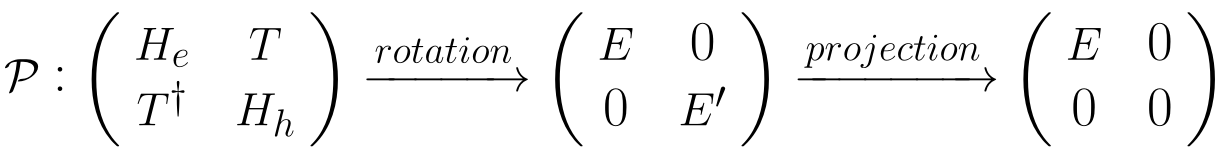
\includegraphics[scale=0.3]{pic6.png}}
\end{center}

The RHS simplifies as
\beq[rhs]
\hat P_{N\sigma}(1-\no) = \fr{1}{2}(1 + \eta + \eta^\dagger)(1-\no) = \fr{1}{2}(1 + \eta^\dagger)(1-\no) && \rr{\because \eta_{N\sigma}(1-\no)=0} \\
\tf \no \ham^\prime \hat P_{N\sigma} (1-\no) = \fr{1}{2}\no \ham^\prime (1+\eta^\dagger_{N\sigma}) (1-\no) = \fr{1}{2}\ham^\prime \eta^\dagger_{N\sigma} && \rr{\because \no \eta^\dagger (1-\no) = \eta^\dagger}
\eeq
The LHS simplifies as
\beq
\no \hml = (\no H_e \no + \no c^\dagger \hat T + \no \hat T^\dagger c + \no H_h (1-\no)) \\
= H_e \no + c^\dagger \hat T \\ 
\rr{\because \no c^\dagger = c^\dagger, \no \hat T^\dagger c = \hat T^\dagger \no c = 0, \no H_h (1-\no) = H_h \no (1-\no) = 0}\\
\eeq
\beq[lhs]
\tf \no \hml \hat P (1-\no) &= \fr{1}{2}(H_e \no + c^\dagger \hat T)(1+\eta^\dagger)(1-\no) \\
&= \fr{1}{2}(H_e \no + H_e \no \eta^\dagger + c^\dagger T + c^\dagger T \eta^\dagger)(1-\no) \\
&= \fr{1}{2}H_e \no \eta^\dagger (1-\no) + c^\dagger T (1-\no) + \fr{1}{2}c^\dagger T \eta^\dagger(1-\no) \\
&= \fr{1}{2}H_e \no \eta^\dagger + \fr{1}{2}c^\dagger T \\
&\rr{\because \eta^\dagger (1-\no) = \eta^\dagger, c^\dagger (1-\no)=c^\dagger, c^\dagger\eta^\dagger = 0}
\eeq
Combining the final equations of \ref{rhs} and \ref{lhs}, we get
\beq
c^\dagger_{N\sigma}\hat T_{N\sigma} + H_e \no \eta^\dagger_{N\sigma} = \ham^\prime \eta^\dagger_{N\sigma}\implies \eta^\dagger_{N\sigma} = \fr{1}{\ham^\prime - H_e \no} c^\dagger_{N\sigma} \hat T_{N\sigma}
\eeq
Defining \(\hat G_e(\hat E_{N\sigma})\) = \fr{1}{\ham^\prime - H_e \no}, 
\beq[etad]
        \eta^\dagger_{N\sigma} = \hat G_e(\hat E_{N\sigma}) c^\dagger_{N\sigma}\hat T_{N\sigma}
\eeq
This expresses the electron-hole transition operator in terms of the eigenblock \(\hat E_{N\sigma}\). \\\\
The expression for \(\eta\) is obtained using \((1-\no)\hml\hat P\no = (1-\no)\ham^\prime \hat P \no\)
\beq
\hat P \no = \fr{1}{2}(1 + \eta+ \eta^\dagger)\no = \fr{1}{2}(\no + \eta) && \rr{\because \eta \no = \eta, \eta^\dagger \no =0}
\eeq
\beq
(1-\no)\hml = (H_h(1-\no)+\hat T^\dagger c)
\eeq
\beq[one]
(1-\no)\hml\hat P\no = \fr{1}{2}H_h (1-\no)\eta +\fr{1}{2}\hat T^\dagger c \no + \fr{1}{2}\hat T^\dagger c\eta = \fr{1}{2}H_h(1-\no)\eta + \fr{1}{2}\hat T^\dagger c \\
\rr{\because c \no = c, c \eta =0}
\eeq
\beq[two]
(1-\no)\ham^\prime\hat P \no = \fr{1}{2}\ham^\prime (1-\no)\eta = \fr{1}{2}\ham^\prime\eta
\eeq
Combining \ref{one} and \ref{two}, we get
\beq
        \eta_{N\sigma} = G_h(\hat E_{N\sigma})  \hat T^\dagger_{N\sigma}c_{N\sigma}
\eeq
where \(G_h(\hat E_{N\sigma} = \fr{1}{\ham^\prime - H_h(1-\no)}\) \\\\

The expression for the eigenblock \(\hat E_{N\sigma}\) is obtained using \(\no \hml \hat P \no = \no \ham^\prime \hat P \no\)
\beq
\no \hml \hat P \no &= \fr{1}{2}(H_e \no + c^\dagger \hat T)(\no + \eta) = \fr{1}{2}\rr{H_e \no + H_e \no \eta + c^\dagger T\no + c^\dagger T \eta} \\
&= \fr{1}{2}\rr{H_e \no + c^\dagger T \eta} \\
&\rr{\because \no \eta =0, c^\dagger \hat T \no = \hat T c^\dagger \no =0} \\
\no \ham^\prime\hat P \no &= \fr{1}{2}\no \ham^\prime (\no + \eta) = \fr{1}{2}\rr{\no \ham^\prime \no + \no \ham^\prime \eta} = \fr{1}{2}\hat E_{N\sigma} \no \\
&\rr{\because \no \ham^\prime \no = \hat E \no, \no \ham^\prime \eta = \ham^\prime \no \eta =0}
\eeq
Combining,
\beq
        \hat E_{N\sigma}\no = H_e \no + c^\dagger_{N\sigma} \hat T_{N\sigma} \eta_{N\sigma}
\eeq
The expression for the lower eigenblock \(\hat E^\prime_{N\sigma}\) is obtained by repeating the last stuff with \(\ham^{\prime\prime}\):
\beq
\hml(1-\hat P) &= \ham^{\prime\prime} (1-\hat P) \\
\implies (1-\no)\hml(1-\hat P)(1-\no) &= (1-\no)\ham^{\prime\prime}(1-\hat P)(1-\no)
\eeq
Now,
\beq
(1-\hat P)(1-\no) = \fr{1}{2}(1-\eta-\eta^\dagger)(1-\no) = \fr{1}{2}\rr{(1-\no)-\eta^\dagger}
\eeq
Therefore,
\beq
(1-\no)\hml(1-\hat P)(1-\no) &= \fr{1}{2}(H_h(1-\no)+\hat T^\dagger c)(1-\no-\eta^\dagger)\\
&= \fr{1}{2}\rr{H_h(1-\no)-\hat T^\dagger c \eta^\dagger} \\
&\rr{\because (1-\no)\eta^\dagger = 0, c(1-\no)=0}\\
(1-\no)\ham^{\prime\prime}(1-\hat P)(1-\no) &= \fr{1}{2}\hat (1-\no)H^{\prime\prime} (1-\no)=\fr{1}{2}\hat E^\prime (1-\no)
\eeq
Combining the last two equations,
\beq[eprime]
        \hat E_{N\sigma}^\prime(1-\no) = H_h(1-\no) - \hat T^\dagger_{N\sigma} c_{N\sigma} \eta^\dagger_{N\sigma}
\eeq

\subsection{Determining the \un}
The starting equation for the above construction was equation \ref{eq1}. That will also provide an expression for the \un. Operating equation \ref{eq1} to the right of \(\ket{1}\) (occupied eigenstate of \no) gives 
\beq
& \hml\hat P_{N\sigma}\ket{1} = \hat E_{N\sigma} \otimes\bf{I}\;\hat P_{N\sigma} \ket{1} = \hat E_{N\sigma} \hat P_{N\sigma} \ket{1} \\
&\implies \hml \un^\dagger \no \un \ket{1} = \hat E_{N\sigma} \un^\dagger \no \un \ket{1} && \rr{\text{substituting expression of \(\hat P_{N\sigma}\)}}\\
&\implies \un \hml \un^\dagger \no \un \ket{1} = \un \hat E_{N\sigma} \un^\dagger \no \un \ket{1} && \rr{\text{operating \(\un\) from left}}\\
&\implies \overline \hml \no \un \ket{1} = \un \hat E_{N\sigma} \un^\dagger \no \un \ket{1}
\eeq
Compare the last equation with \ref{Hdiag}. In order to satisfy the first equation of \ref{Hdiag}, we need the following two equations,
\beq[ucond]
\no \un \ket{1} &\propto \ket{1} \\
\un \hat E_{N\sigma} \un^\dagger &=  E_{N\sigma}
\eeq
The second equations says 
\beq[Ecomm]
\qq{E_{N\sigma},\un}=0
\eeq
The \(\un\) that satisfies the first equation is \(\un = \kappa\rr{1-\hat\eta+\hat\eta^\dagger}\). \(\kappa\) is a constant determined by the unitarity condition \(\un\un^\dagger=\bf{I}\). To check that this satisfies \ref{ucond},
\beq
\hat n_{N\sigma}\hat U_{N\sigma}\ket{1} &\propto \hat n_{N\sigma}(1-\hat \eta + \hat \eta^\dagger)\ket{1} \\
&= \hat n_{N\sigma}(1-\hat \eta)\ket{1} && \rr{\eta^\dagger \ket{1}=0} \\
&= \ket{1} - \hat n \hat \eta\ket{1} \\
&= \ket{1} && \rr{\hat n \hat \eta = 0}
\eeq
To find \(\kappa\), we will use the unitarity of \il{\hat U_{N\sigma}}:
\beq
\un\un^\dagger 	&=\kappa^2(1-\eta+\eta^\dagger)(1+\eta-\eta^\dagger) \\
&= \kappa^2(1+\cc{\eta,\eta^\dagger}) && \rr{\eta^2 = {\eta^\dagger}^2 = 0} \\
&= 2\kappa^2 && \rr{\cc{\eta,\eta^\dagger}=1}\\
\implies \kappa=\fr{1}{\sqrt{2}}
\eeq

\beq[uni]
\un = \fr{1}{\sqrt{2}}\rr{1-\hat\eta+\hat\eta^\dagger}
\eeq

\subsection{Summary of the results}
\begin{itemize}
	\item \(\eta^\dagger = G_e c^\dagger T \)
	\item \(\eta^\dagger = G_h T^\dagger c\)
	\item \(\eta^\dagger \eta = \hat n\)
	\item \(\eta \eta^\dagger = 1-\hat n\)
	\item \(U = \fr{1}{\sqrt 2}\rr{1-\eta+\eta^\dagger}\)
\end{itemize}

\subsection{A Simple Example}
\beq
\ham = -t\rr{c^\dagger_2c_1+c^\dagger_1c_2}+V\hat n_1\hat n_2-\mu(\hat n_1+\hat n_2) && \hat n_i = c^\dagger_i c_i = \begin{pmatrix} V-2\mu & 0 & 0 & 0 \\
0 & -\mu & -t & 0 \\ 0 & -t & \mu & 0 \\ 0 & 0 & 0 & 0 \\
\end{pmatrix}
\eeq
The basis used is the ordered set \{\(\ket{11}, \ket{10}, \ket{01}, \ket{00}\)\} \\\\
For this problem, we take \(N\sigma\equiv1\). 1 refers to the first site. First step is to represent the Hamiltonian in block matrix form (equation \ref{h}).
\beq
\hat H_{1,e} &= Tr_1[\ham\hat n_1] \\
&= Tr_1[V\hat n_1\hat n_2-\mu(\hat n_1+\hat n_2)] && \rr{\text{\(c\) and \(c^\dagger\) will not conserve the eigenvalue of \(\hat n\)}} \\
&= V\hat n_2 -\mu(1+\hat n_2) &&\rr{Tr_1[V\hat n_1 \hat n_2]=VTr_1[\hat n_1]\hat n_2=V\hat n_2}\\
&= (V-2\mu)\hat n_2 -\mu(1-\hat n_2)
\eeq
Next is calculation of \(\hat H_{1,h}\):
\beq
\hat H_{1,h} &= Tr_1[\ham(1-\hat n_1)] = -\mu\hat n_2\\
\eeq
Next is calculation of \(T_{1,e-h}\).
\beq
T_{1,e-h} &= Tr_1[\ham c_1] \\  
&= Tr_1[-tc^\dagger_1c_2c_1] = -tc_2 && \rr{\text{the only term that conserves eigenvalue of \(\hat n\)}}
\eeq
Therefore, \(T^\dagger_{1,e-h} = -tc^\dagger_2\). The block matrix form becomes 
\beq[bmf]
\ham = 	\begin{pmatrix}
        (V-2\mu)\hat n_2 -\mu(1-\hat n_2) & -tc_2 \\
		-tc^\dagger_2 & -\mu\hat n_2 \\
		\end{pmatrix}
\eeq
The block-diagonal form is, as usual, \(\overline\ham = \begin{pmatrix}
		\hat E_1 & 0 \\
		0 & \hat E^\prime_1 \\
		\end{pmatrix} \) \\
The expression of \(\eta^\dagger\) is \(\hat \eta^\dagger = \hat G_e c_1^\dagger \hat T_{1,e-h} = G_e c^\dagger_1 (-t c_2)\) . Hence, \(\eta = -t c^\dagger_2 c_1 G_e^\dagger\). Since \(H_e ^\dagger = H_e\) for this problem, we have \(\eta = -t c_2^\dagger c_1 G_e\). It was proved in the formalism that \(\eta^\dagger \eta = \hat n_1\). Therefore,
\beq
t^2 G_e c_1^\dagger c_2 c_2^\dagger c_1 G_e = \hat n_1 &\implies t^2 \hat n_1 (1-\hat n_2) = \hat n_1 \{G_e^{-1}\}^2 = \hat n_1 (\ham^\prime - H_e\hat n_1)^2 \\
&\implies t^2 \hat n_1^2 (1-\hat n_2)^2 = (\ham^\prime \hat n_1 - H_e \hat n_1)^2 \\
&\implies \ham^\prime \hat n_1 = H_e \hat n_1 + t\hat n_1 (1-\hat n_2)=(V-2\mu)\hat n_1 \hat n_2 +(t- \mu)\hat n_1(1-\hat n_2) 
\eeq
This equation gives the upper block of the diagonalised Hamiltonian. Why the upper block? Because it is multiplied by \(\hat n_1\), and hence can give non-zero contribution only in the upper block. It is also obvious that the upper block itself is internally diagonal in \(\hat n_2\); this is seen from the fact that the expression of \(\ham^\prime \hat n_1\) has no \(c_2\) or \(c^\dagger_2\), only \(\hat n_2\). The term multiplying \(\hat n_2\) becomes the upper matrix element in the block of \(\hat n_2\), while that multiplying \(1-\hat n_2\) becomes the lower element. Summarizing,
\beq
\overline \ham = \ham^\prime \hat n_1 + \ham^{\prime\prime}(1-\hat n_1) = \begin{pmatrix} {\begin{matrix} V-2\mu & 0 \\ 0 & t-\mu \end{matrix}} & & \bf{0}_{2x2} & & \\ \bf{0}_{2x2} & & (\hat E^\prime_1)_{2x2} & & \end{pmatrix}
\eeq
The \(\hat E^\prime\) is the contribution from \(\ham^{\prime\prime}\); just as \(\ham\hat n_1\) gives the upper block contribution, \(\ham^{\prime\prime}\) gives the lower contribution. And since \(\ham^{\prime\prime} = \begin{pmatrix} \hat E^\prime & 0 \\ 0 & \hat E^\prime\end{pmatrix}\), we end up with \(\hat E^\prime\) in the lower block of \(\overline \ham\). It still remains to compute \(\ham^{\prime\prime} (1-\hat n_1) = \hat E^\prime(1-\hat n_1)\). But that is easy because we already have the expression for that, equation \ref{eprime}.
\beq
E^\prime_1(1-\hat n_1) = H_h(1-\hat n_1) - \hat T^\dagger_1 c_1 \eta^\dagger = -\mu (1-\hat n_1)\hat n_2 - t^2 c_2^\dagger c_1 G_e c_1^\dagger\hat c_2
\eeq
This is the expression for the lower block. But to get the final matrix elements, we need to resolve it in \(\hat n_2\). That is, the upper matrix element of the lower block will be \(\bra{01}E^\prime(1-\hat n_1)\ket{01}\) and the lower element will be \(\bra{00}E^\prime(1-\hat n_1)\ket{00}\). The bra and ket are written in the notation \(\bra{n_1,n_2},\ket{n_1,n_2}\). Since this is the lower block in the representation of \(\hat n_1\), \(n_1\) will always be zero while calculating the elements of \(\hat E^\prime\). \(n_2=1(0)\) means the upper(lower) diagonal element. Similarly,  \(\bra{01}E^\prime(1-\hat n_1)\ket{00}\) is an off-diagonal element. \\\\
It is easy to see that the off-diagonal terms will be zero. The lower diagonal term will also be zero: \(\hat n_2\ket{n_1, 0} = c_2 \ket{n_1, 0} = 0\). Thus the only non-zero term is
\beq
\bra{01}E^\prime(1-\hat n_1)\ket{01} = -\mu -t^2\bra{10}G_e\ket{10}
\eeq
Now,
\beq
\bra{10}G_e^{-1}\ket{10}=&\bra{10}H^\prime - (V-\mu)\hat n_1\hat n_2 + \mu \hat n_1 \ket{10} \\ &= \bra{10}\ham^\prime\ket{10} + \mu = \bra{10}\ham^\prime\hat n_1\ket{10} + \mu \\
&=\bra{10}(V-2\mu)\hat n_1 \hat n_2 +(t- \mu)\hat n_1(1-\hat n_2)\ket{10} + \mu \\
&= t -\mu +\mu = t \\
\tf \bra{10}G_e\ket{10} &= \fr{1}{t}
\eeq
Therefore, \(\bra{01}E^\prime(1-\hat n_1)\ket{01} = -\mu -t^2\fr{1}{t} = -\mu -t\).
The final diagonalized matrix becomes 

\beq
\overline \ham &= \bordermatrix{
               	~ & \ket{11} & \ket{10} & \ket{01} & \ket{00} \cr
               	& (V-2\mu) & 0 & 0 & 0 \cr \\
               	& 0 & (t-\mu) & 0 & 0 \cr \\
               	& 0 & 0 & -(\mu+t) & 0 \cr \\
               	& 0 & 0 & 0 & 0 \cr
               	}
\eeq

There's an alternative way of deriving the lower block - using the fact that the trace is invariant under the URG transformations. First note that in the original Hamiltonian, only the upper \(3\times3\) portion is interacting among themselves, the 4\uu{th} row and 4\uu{th} column of the Hamiltonian do not interact with the rest. This means that the lower element of \(\hat E^\prime\) is zero. Also note that the unitary transformations do not alter the partial trace of the matrix. Specifically,
\beq
Tr_1\rr{\overline \ham} = Tr_1\rr{\un \ham \un^\dagger} = Tr_1\rr{\un^\dagger \un \ham} = Tr_1\rr{\ham}
\eeq
Since we know the expression of \(\hat E_1\) and the structure of \(\hat E^\prime_1\), we can write down the structure of \(\overline \ham\):

\beq
\overline \ham = 
\begin{pmatrix}
        V-2\mu  &       &       & \\
                & t-\mu &       & \\
                &       & \hat E^\prime_1 & \\
                &       &       &       0
\end{pmatrix}
\eeq

Therefore, 
\(Tr_1\overline \ham = (V-2\mu)\hat n_2 + (t-\mu)(1-\hat n_2) + \hat E^\prime_1\hat n_2\). From equation \ref{bmf}, \(Tr_1\rr{\ham} = V\hat n_2 - \mu(1+\hat n_2) - \mu \hat n_2\). Equating the two traces, we get an expression for the lower block:

\beq
\hat E_1^\prime\hat n_2 = -(\mu+t)\hat n_2
\eeq

We thus get the same final Hamiltonian.

\subsubsection{The Eigenstates}
The unitarily transformed Hamiltonian, \(\overline \ham\) is diagonal in the basis of \(\hat n\). This implies that the eigenstates of the original Hamiltonian \(\ham\) are the unitarily transformed versions of the eigenkets of \(\hat n\):
\beq
\ham (\un^\dagger \ket{n_1,n_2}) = \un^\dagger \overline \ham \ket{n_1,n_2} = \un^\dagger E_{n_1,n_2}\ket{n_1,n_2} = E_{n_1,n_2}(\un^\dagger\ket{n_1,n_2})
\eeq
To find the eigenvectors \(\un^\dagger\ket{n_1,n_2}\), we need to find the \(\un\). From equation \ref{uni}, we have \(\un = \fr{1}{\sqrt 2}\rr{1+\hat \eta^\dagger - \hat \eta}\). 

We have  \(\hat \eta_{1} = G_h T^\dagger c_1\). Using the expression of \(\hat E_1\). this simplifies as:
\beq
        \eta &= \fr{1}{\hat E_1 - H_h}(-tc^\dagger_2)c_1 = \fr{-t}{(V-2\mu)\hat n_2 + (t-\mu)(1-\hat n_2)+\mu \hat n_2}c_1c_2^\dagger = \fr{-t}{V-\mu}c_1 c^\dagger_2 \\
        \eta^\dagger &= c_1^\dagger \fr{1}{(V-2\mu)\hat n_2 +(t-\mu)(1-\hat n_2)-(V-2\mu)\hat n_2 + \mu(1-\hat n_2)}(-tc_2) = - c_1^\dagger c_2
\eeq

\beq
        \tf \un &= \fr{1}{\sqrt 2} \qq{1+\fr{t}{V-\mu}c_1 c^\dagger_2-c_1^\dagger c_2} \implies \un^\dagger = \fr{1}{\sqrt 2}\qq{1+\fr{t}{V-\mu}c_1^\dagger c_2 - c_2 c^\dagger_1}
\eeq

To get the eigenstates of \ham, I act with \(U^\dagger\) on the eigenstates (\(\ket{n_1,n_2}\)):
\beq
        \un ^\dagger \ket{11} = \ket{11}
\eeq
\beq
        \un ^\dagger \ket{00} = \ket{00}, \\
\eeq
\beq
\un ^\dagger \ket{10} = \fr{1}{2}\rr{\ket{10}-\eta\ket{10}} = \fr{1}{2}\rr{\ket{10}+t c_2^\dagger c_1 \hat G_e \ket{10}} = \fr{1}{2}\rr{\ket{10}+tc_2^\dagger c_1 \fr{1}{t} \ket{01}} \\ = \fr{1}{2}\rr{\ket{10}+\ket{01}}
\eeq
\beq
        \un^\dagger\ket{01} = \fr{1}{2}\rr{\ket{01}+\eta^\dagger\ket{01}} = \fr{1}{2}\rr{\ket{01} - t \hat G_e c_1^\dagger c_2 \ket{01}} = \fr{1}{2}\rr{\ket{01} - \ket{10}}
\eeq
The eigenstates come out to be (upto a normalizaiton):
\beq
        &\ket{00} \\
        &\ket{10} + \ket{01} \\
        &\ket{01} - \ket{10} \\
        &\ket{11} \\
\eeq


\newpage
\section{Applying the RG on the Hubbard dimer (real space)}
\begin{gather}
\ham = -t\sum_\sigma(c_{1\sigma}^\dagger c_{2\sigma}+c_{2\sigma}^\dagger c_{1\sigma})+U\rr{\na\nb+\nc\nd}
\end{gather}
We begin by decoupling the first degree of freedom, namely, a spin-up electron on the first site. 
\begin{gather}
        H^e_{1\ua} = Tr_{\na}(\ham\na) = U(\nb+\nc\nd)-t(\cb^\dagger\ce+\ce^\dagger\cb) \\  
        H^h_{1\ua} = Tr_{\na}(\ham(1-\na)) = U\nc\nd - t(\cb^\dagger\ce+\ce^\dagger\cb) \\
        T_{1\ua} = Tr_{\na}(\ham\ca) = -t\cd\\
        T^\dagger_{1\ua} = Tr_{\na}(\ca^\dagger\ham) = -t\cd^\dagger
\end{gather}
Assume that the Hamiltonian, after block-diagonalization in the subspace of \il{\na}, looks like
\beq
\ol \ham = U^\dagger_{1\ua} \ham U_{1\ua} = \begin{pmatrix} \hat E_{1\ua} & 0 \\ 0 & \hat E^\prime_{1\ua} \end{pmatrix}
\eeq
\il{\hat E_{1\ua}} and \il{\hat E^\prime_{1\ua}} are the sub-Hamiltonians with one fewer degree of freedom. That is, they are the Hamiltonians in the subspaces \il{\na=1,0} respectively.\\
\subsection{\il{\na=1}}
Define \il{\hat H^\prime_{1\ua} \equiv \hat E_{1\ua}\otimes \mathbb{I}}. Again, proceeding as in the formalism, we can derive
\begin{gather}
        \eta_{1\ua} = \hat G_e \hat T_{1\ua}^\dagger c_{1\ua} \\
        \eta^\dagger_{1\ua} = \hat G_h c_{1\ua}^\dagger\hat T_{1\ua}
\end{gather}


The process of finding the eigenvalues involves using the equations for \il{\eta^\dagger\eta} and \il{\eta\eta^\dagger}:
\begin{gather}
        \eta^\dagger_{1\ua} \eta_{1\ua} = \na \label{2} \\
        \eta_{1\ua} \eta^\dagger_{1\ua} = 1-\na \label{1}
\end{gather}
This subspace involves \il{1-\na=0}, hence we cannot use eq.~\ref{1}. We also have the choice of starting with the expression of either \il{\eta} or \il{\eta^\dagger}, but since \il{\eta} involves \il{1-\na} in the denominator, it doesn't lead to anything fruitful. So we start with \il{\eta^\dagger_{1\na}}. Using eq.~\ref{etad}:
\beq
 \eta^\dagger_{1\ua} = G_e c_{1\ua}^\dagger T_{1\ua} = -t \hat G_e c^\dagger_{1\ua}c_{2\ua} = \fr{-t}{\hat E_{1\ua}\na -H_e \hat n_{1\ua}}c^\dagger_{1\ua}c_{2\ua}
\eeq
The hole to electron operator \il{\eta_{1\ua}} is obtained by taking the Hermitian conjugate of \il{\eta^\dagger_{1\ua}}:
\beq[eta1]
 \eta_{1\ua} = c^\dagger_{2\ua}c_{1\ua}\fr{-t}{\hat E_{1\ua}\na -H_e \hat n_{1\ua}}
\eeq
Here we used the fact that \il{H_e\na} is Hermitian as seen from its expression, and

\il{\hat E_{1\na}\na\equiv\hat E_{1\na}\otimes\na} is Hermitian because it is a sub-Hamiltonian by definition. Substituting these expressions in eq.~\ref{2},
\begin{gather}
\hat n_{1\ua}=\eta_{1\ua}^\dagger\eta_{1\ua}=\fr{-t}{\hat E_{1\ua}\na -H_e \hat n_{1\ua}}\na(1-\nc)\fr{-t}{\hat E_{1\ua}\na -H_e \hat n_{1\ua}}\\
        \implies (\hat E_{1\ua}\na -H_e \hat n_{1\ua})^2 = t^2\na(1-\nc)\label{cent}
\end{gather}
This is the central equation(eq.~\ref{cent}) that will  be used for determining all the eigenvalues for the \il{\na=1} subspace. Substituting the expression for \il{H_e} gives:
\beq[work]
\qq{\hat E_{1\ua}\na -U\na\nb -U\nc\nd\na +t(\cb^\dagger\ce+\ce^\dagger\cb)\na}^2 = t^2\na(1-\nc)
\eeq
\subsection{N = 2}
We first look  at the \il{N=2} portion of the \il{\na} occupied subspace. The remaining degrees of freedom are \il{\nb}, \il{\nc} and \il{\nd}. Notice that the working equation, eq.~\ref{work} involves the creation and annihilation operators only for \il{\nb} and \il{\nd}. This means that \il{\nb} and \il{\nd} form a coupled degree of freedom, and this is in turn decoupled from \il{\nc}.Out of the two electrons (\il{N=2}), one electron is already there at \il{\na}. This leaves us with two possible subspaces to work in:
\begin{itemize}
    \item\il{\mathcal{\hat P} = \ket{1100}\bra{1100}+\ket{1001}\bra{1001}} \\\\
        This is the subspace in which we keep \il{\nc} empty, and the second electron thus lie somewhere in the subspace spanned by \il{\nb} and \il{\nd}. The notation is obvious: \il{\ket{1100}\equiv\ket{\ua\da,0}} and \il{\ket{1001} \equiv \ket{\ua,\da}}. In this subspace, the right hand side of eq.~\ref{work} is unity, because \il{\na=1} and \il{\nc=0}. Define \il{\hat a_x = \begin{pmatrix}0 & 1 \\ 1 & 0\end{pmatrix}}. Clearly, \il{\hat a_x^2=1}. Then, in this subspace,
\begin{gather}
\qq{\hat E_{1\ua}\na -U\na\nb -U\nc\nd\na +t(\cb^\dagger\ce+\ce^\dagger\cb)\na}^2 = t^2 \hat a_x^2 \\
\implies \hat E_{1\ua}\na -U\na\nb -U\nc\nd\na +t(\cb^\dagger\ce+\ce^\dagger\cb)\na = \pm t \hat a_x
\end{gather}
Next we need to write the LHS in this subspace. Taking \il{\ket{1100}} and \il{\ket{1001}} as the basis elements, we see that both \il{\ce^\dagger\cb} and \il{\cb^\dagger\ce} take one basis vector to the other, and hence
\beq
\cb^\dagger\ce+\ce^\dagger\cb = \begin{pmatrix} 0 & -1 \\ -1 & 0 \end{pmatrix}
\eeq
\begin{minipage}{\textwidth/2}
Since \il{\nc=0}, the \il{\nc\nd\na} term drops out. Also,
\beq
\na\nd=\begin{pmatrix} 1 & 0 \\ 0 & 0\end{pmatrix}
\eeq
Finally, \il{\hat E_{1\ua,2} \equiv \mathcal{P}\hat E_{1\ua}\mathcal{P}} is the projected Hamiltonian in this subspace. Putting all these together,
\end{minipage}
\hspace*{60pt}
\begin{minipage}{\textwidth/3}
	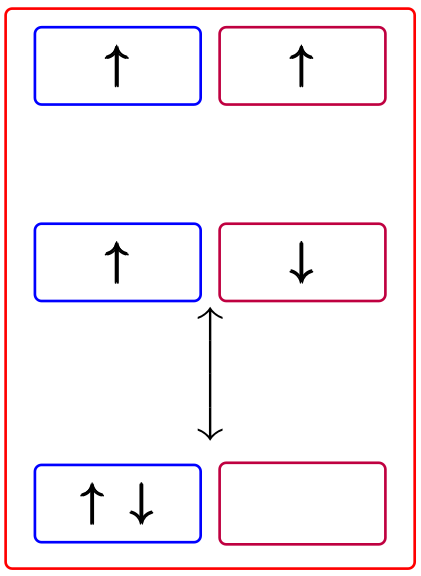
\includegraphics[scale=0.3]{pic1.png}
\end{minipage}
\begin{gather}
\hat E_{1\ua,2} - \begin{pmatrix} U & 0 \\ 0 & 0 \end{pmatrix} - \begin{pmatrix}0 & t \\ t & 0 \end{pmatrix} = \pm \begin{pmatrix} 0 & t \\ t & 0 \end{pmatrix}\\
\implies \hat E_{1\ua,2} = \begin{pmatrix} U & 0  \\ 0 & 0 \end{pmatrix} , \begin{pmatrix} U & 2t \\ 2t & 0 \end{pmatrix}
\end{gather}
The first matrix gives eigenvalues \il{=\{U, 0\}} and eigenvectors \il{=\{\ket{\ua\da,0}, \ket{\ua,\da}\}}. The second matrix gives eigenvalues \il{E_\pm=\fr{U\pm\sqrt{U^2+16t^2}}{2}} and eigenvectors \il{=\{2t\ket{\ua,\da}+E_\pm\ket{\ua\da,0}\}}. Note that this is not the eigenvector for the total Hamiltonian, because it doesn't include the contribution from \il{\na=0} sector.
\item \il{
        \mathcal{P} = \ket{1010}\bra{1010}} \\\\
In the previous subspace, we set \il{\nc=0}, so here we consider \il{\nc=1}:
Since \il{\nb=\nd=0}, we have \il{U(\na\nb+\nc\nd)=0} and \il{\cb^\dagger\ce+\ce^\dagger\cb = 0}. The RHS is also zero. This means that in this subspace, the only eigenvalue is \il{E=0}. The eigenvector is \il{\ket{\ua,\ua}}.
\end{itemize}

\subsection{N = 1}
This case is simpler, because the only electron is placed at \il{\na}. Thus, \il{\nb=\nc=\nd=0} in this subspace. Since the subspace has just one state, it is unidimensionl, and the equation for this subspace will involve scalars instead of matrices. The RHS is hence \il{t^2} instead of \il{t^2a_x^2}. Since there are no electrons in \il{\nb} or \il{\nd}, the creation and annihilation operators in the LHS are zero:
\beq
\na\nb+\nc\nd = \cb^\dagger\ce+\ce^\dagger\cb = 0
\eeq
Eq.~\ref{work} thus reduces to
\beq[En1]
\hat E_{1\ua,1} = \pm t
\eeq
\il{\hat E_{1\ua,1}} is the projected Hamiltonian in this subspace. The eigenvalues in this subspace come out to be \il{\pm t}. Since the only state in this subspace is \il{\ket{\ua,0}}, that is the contribution to the eigenvectors.

\subsection{N = 3}

With one electron at \il{\na}, we have two electrons to place. There are two options:
\begin{itemize}
    \item \il{
            \mathcal{\hat P} = \ket{1110}\bra{1110}+\ket{1011}\bra{1011}}\\\\
    Since the equation is diagonal in \il{\nc}, it makes sense to place one electron at \il{\nc}, and the other electron in the coupled subspace, that is, \il{\nb} and \il{\nd}. The corresponding projection operator is
The RHS of eq.~\ref{work} in this subspace is 0, because \il{\nc=1}. This also means that
\begin{gather}
\na\nb+\nc\nd\na=\nb+\nd=\begin{pmatrix} 1 & 0 \\ 0 & 1 \end{pmatrix}\\
\cb^\dagger\ce+\ce^\dagger\cb = \begin{pmatrix} 0 & 1 \\ 1 & 0 \end{pmatrix}
\end{gather}
The equation becomes
\beq
\hat E_{1\ua,3} - \begin{pmatrix} U & 0 \\ 0 & U \end{pmatrix}+\begin{pmatrix} 0 & t \\ t & 0 \end{pmatrix}=0 \implies \hat E_{1\ua,3} = \begin{pmatrix} U & -t \\ -t & U \end{pmatrix}
\eeq
The eigenvalues come out as \il{U\pm t}. The eigenvectors are \il{\ket{1110}\mp\ket{1011}}.
\item \il{\mathcal{\hat P} = \ket{1101}} \\\\
    The other sensible choice is to keep \il{\nc=0}. Since this subspace has just one state, it is unidimensional, and the equation is scalar.
        \beq
            \na\nb+\nc\nd = 1 \\
            \cb^\dagger\ce+\ce^\dagger\cb=0 \\
            \hat E_{1\ua,3} - U = \pm t
        \eeq
        The eigenvalues are \il{U\pm t}, and the eigenvector is \il{\ket{\ua\da,\da}}.
\end{itemize}
\subsection{\il{\na=0}}
To calculate the eigenvalues for the unoccupied sector, define \il{\ham^{\prime\prime}  \equiv \hat E^\prime_{1\na} \otimes \mathbb{I}}. We can derive
\begin{gather}
    \eta_{1\ua} = -\hat G_h^\prime \hat T_{1\ua}^\dagger c_{1\ua}\label{now} \\
        \eta^\dagger_{1\ua} = -\hat G_e^\prime c_{1\ua}^\dagger\hat T_{1\ua}\label{etad2}\\
        \eta^\dagger_{1\ua}\eta_{1\ua}=\na \\
        \eta_{1\ua}\eta^\dagger_{1\ua}=1-\na\label{zero}
\end{gather}

Note that \il{\hat G^\prime} involves \il{\hat E^\prime} in the denominator, because we now want to diagonalize the unoccupied block. Since \il{\na=0} now, we need to use eq.~\ref{zero} and start with the expression of \il{\eta_{1\ua} (eq.~\ref{now})} instead of \il{\eta^\dagger_{1\ua}}. Substituting the expression for \il{\eta_{1\ua}} and it's conjugate gives the following equation for the unoccupied sector:
\beq
\qq{\hat E^\prime_{1\ua} - U\nc\nd + t(\cb^\dagger\ce+\ce^\dagger\cb)}^2 = t^2 \nc
\eeq

\subsection{N = 1}

With no electron on \il{1,\ua}, the only electron can reside in a superposition of \il{\ket{\da,0}} or \il{\ket{0,\da}}:
\begin{gather}
    \mathcal{P} = \ket{0100}\bra{0100} + \ket{0001}\bra{0001}
\end{gather}
The right hand side is zero because \il{\nc=0}. Also,
\begin{gather}
    \na\nb+\nc\nd = 0\\
    \cb^\dagger\ce+\ce^\dagger\cb = \begin{pmatrix} 0 & t \\ t & 0 \end{pmatrix}
\end{gather}
Putting it all together,
\begin{gather}
    \rr{E^\prime_{1\ua,2}+ \begin{pmatrix} 0 & t \\ t & 0 \end{pmatrix}}^2 = 0 \\
    \implies E^\prime_{1\ua,2}= \begin{pmatrix} 0 & -t \\ -t & 0 \end{pmatrix}\label{eval}
\end{gather}
The eigenvalues are \il{\pm t}, the eigenvectors are \il{\ket{\da,0}\mp\ket{0.\da}}. 

\subsection{N = 2}

\begin{gather}
        \mathcal{P} = \ket{0110}\bra{0110}+\ket{0011}\bra{0011} \\
        \implies E^\prime_{1\ua,2}-\begin{pmatrix} 0 & 0 \\ 0 & U \end{pmatrix} - \begin{pmatrix} 0 & t \\ t & U \end{pmatrix} = \pm t a_x \\
                \implies E^\prime_{1\ua,2} = \begin{pmatrix} 0 & 0 \\ 0 & U \end{pmatrix}, \begin{pmatrix} 0 & 2t \\ 2t & 0 \end{pmatrix}
\end{gather}
The eigenvalues are \il{0, U} for the first matrix, with eigenvectors \il{\ket{0110}, \ket{0011}}, and\\  \il{E_\pm=\fr{U\pm\sqrt{U^2+16t^2}}{2}},  and \il{2t\ket{\da,\ua}+E_\pm\ket{0,\ua\da}} for the second.\\\\
Similar to the \il{\na=1} situation,we can consider another subspace where \il{\nc=0}:
\beq
\mathcal{P} = \ket{0101}\bra{0101}
\eeq
Obviously, \il{\na\nb+\nc\nd=\cb^\dagger\ce+\ce^\dagger\cb=0}. The only eigenvalue is 0, with eigenvector \il{\ket{\da,\da}}.

\subsection{N = 3}

Only state in this subspace is \il{\ket{0111}}.
\begin{gather}
    \mathcal{P} = \ket{0111} \\
    \na\nb+\nc\nd = 1 \\
    \cb^\dagger\ce+\ce^\dagger\cb = 0
\end{gather}
The equation(scalar) in this subspace is 
\begin{gather}
    E^\prime_{1\ua,3}-U = \pm t\label{yeah}
\end{gather}

The eigenvalues are \il{U\pm t}. The eigenvector is \il{\ket{0111}}.

\begin{center}
	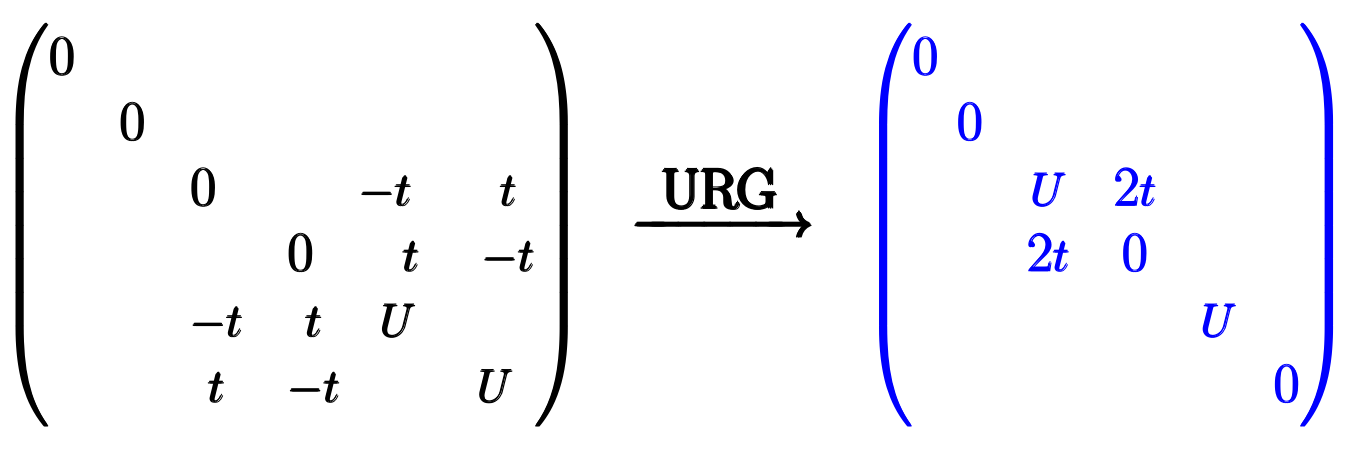
\includegraphics[scale=0.3]{pic2.png}
\end{center}

\subsection{The eigenstates}
The eigenstates obtained for the various subspaces form only parts of the total eigenstates. Using the unitary operator \il{\hat U^\dagger = \fr{1}{\sqrt 2}(1+\eta-\eta^\dagger)}, these individual eigenstates can be combined into the total eigenstates.

\subsubsection{N = 1}

First, consider the case of \il{\na=1}. The eigenstate for the subspace is \il{\ket{\na=1,N=1}=\ket{\ua,0}}. The total eigenstates are given by \il{\ket{\psi} = \hat U^\dagger_{1\ua} \ket{\na=1,N=1}}. Note that since \il{\eta^\dagger_{1\ua}} takes a hole at \il{\na} to an electron at the same quantum number, and since there is no hole at that quantum number (\il{\na} is occupied), \il{\eta^\dagger} will act to give zero, so we drop it.
\beq
\hat U_{1\ua}^\dagger \ket{\na=1,N=1} = \fr{1}{\sqrt 2} (1+\eta_{1\ua})\ket{\ua,0}
\eeq
From eq.~\ref{eta1}, \il{\eta_{1\ua} = c^\dagger_{2\ua}c_{1\ua}\fr{-t}{\hat E_{1\ua}\na -H_e \hat n_{1\ua}}}. In the subspace we are talking about, \\\il{\hat E_{1\ua}\na -H_e \hat n_{1\ua}=\pm t} (see eq.~\ref{En1}). Therefore,
\beq
\eta_{1\ua}\ket{\ua,0} = \mp \cd^\dagger\ca \ket{\ua,0}= \mp \ket{0,\ua}
\eeq
The total eigenstate turns out to be
\beq
\hat U_{1\ua}^\dagger \ket{\na=1,N=1} = \fr{1}{\sqrt 2}(\ket{\ua,0}+\eta_{1\ua}\ket{\ua,0}) = \ket{\ua,0} \mp \ket{0,\ua}
\eeq
Note that the respective eigenvalues are \il{\pm t}. \\\\
Now consider the case of \il{\na=0}. The eigenstates for the subspace is \\\il{\ket{\na=0, N=1} = \ket{\da,0}\mp\ket{0,\da}}. This time, however, since the states are missing an electron in \na, \il{\eta} will act trivially, and we are left with
\beq
\hat U_{1\ua}^\dagger \ket{\na=0, N=1} = \fr{1}{\sqrt 2}(1-\eta^\dagger_{1\ua})\ket{\na=0, N=1}
\eeq
From eq.~\ref{now}, \il{\eta^\dagger_{1\ua} = -\ca^\dagger\cd\hat G^\prime_h = \ca^\dagger\cd \fr{t}{E^\prime - H_h(1-\na) }}. Note, however, that \il{\ket{\na=0,N=1}} does not have any electron at \nc, and \il{\cd} in \il{\eta^\dagger_{1\ua}} will necessarily give 0. Therefore,
\beq
\eta^\dagger_{1\ua}\ket{\na=0, N=1} = 0
\eeq
which means
\beq
U_{1\ua}^\dagger \ket{\na=0, N=1} = \fr{1}{\sqrt 2}\ket{\na=0, N=1} = \fr{\ket{\da,0}\mp\ket{0,\da}}{\sqrt 2}
\eeq
These are thus the final eigenstates for respective eigenvalues \il{\pm t}.\\
The four eigenstates for \il{N=1} are listed in this table:
\begin{center}
\begin{tabular}{|c|c|}
 \hline
    \il{t}  & \il{\fr{\ket{\ua,0} - \ket{0,\ua}}{\sqrt 2}} \\
    \il{-t} & \il{\fr{\ket{\ua,0} + \ket{0,\ua}}{\sqrt 2}} \\
    \il{t}  & \il{\fr{\ket{\da,0} - \ket{0,\da}}{\sqrt 2}} \\
    \il{-t} & \il{\fr{\ket{\da,0} + \ket{0,\da}}{\sqrt 2}} \\
 \hline
\end{tabular}
\end{center}

\subsubsection{N = 3}

The eigenstate for the first subspace are \\\il{\ket{\na=1,N=3}=\ket{\ua\da,\ua}\mp\ket{\ua,\ua\da}}. The total eigenstates are given by \il{\hat U^\dagger_{1\ua} \ket{\na=1,N=3}}. Note that since \il{\eta^\dagger_{1\ua}} takes a hole at \il{\na} to an electron at the same quantum number, and since there is no hole at that quantum number (\il{\na} is occupied), \il{\eta^\dagger} will act to give zero, so we drop it.
\beq
\hat U_{1\ua}^\dagger \ket{\na=1,N=3} = \fr{1}{\sqrt 2} (1+\eta_{1\ua})(\ket{\ua\da,\ua}\mp\ket{\ua,\ua\da})
\eeq
From eq.~\ref{eta1}, \il{\eta_{1\ua} = c^\dagger_{2\ua}c_{1\ua}\fr{-t}{\hat E_{1\ua}\na -H_e \hat n_{1\ua}}}. Since the part before \il{\ca} can only attach a coefficient to the kets, and since \il{\cd^\dagger} will act on both \il{\ket{\ua\da,\ua}} and \il{\ket{\ua,\ua\da}} to give zero, we have
\beq
\eta_{1\ua}\ket{\na=1,N=3}=0 
\eeq
The total eigenstates turn out to be
\beq
\hat U_{1\ua}^\dagger \ket{\na=1,N=3} = \fr{1}{\sqrt 2}\ket{\na=1,N=3}+\eta_{1\ua}\ket{\na=1,N=3} = \fr{\ket{\ua\da,\ua}\mp\ket{\ua,\ua\da}}{\sqrt 2}
\eeq
Note that the respective eigenvalues are \il{U \pm t}. \\\\
Now consider second subspace for \il{N=3,\na=1}. The eigenstate is \il{\ket{\ua\da,\da}}. Here, \il{E-H_e = \pm t}, therefore,
\beq
\eta_{1\ua}\ket{\ua\da,\da} = \cd^\dagger\cb\fr{-t}{\pm t} \ket{\ua\da,\da} = \mp \ket{\da,\ua\da}
\eeq
which means
\beq
U_{1\ua}^\dagger \ket{\ua\da,\da} = \fr{\ket{\ua\da,\da}\mp\ket{\da,\ua\da}}{\sqrt 2}
\eeq
These are thus the final eigenstates for respective eigenvalues \il{U\pm t}.\\
The four eigenstates for \il{N=1} are listed in this table:
\begin{center}
\begin{tabular}{|c|c|}
 \hline
    \il{U+t}    & \il{\fr{\ket{\ua\da,\ua} - \ket{\ua,\ua\da}}{\sqrt 2}} \\
    \il{U-t}    & \il{\fr{\ket{\ua\da,\ua} + \ket{\ua,\ua\da}}{\sqrt 2}} \\
    \il{U+t}    & \il{\fr{\ket{\ua\da,\da}-\ket{\da,\ua\da}}{\sqrt 2}} \\
    \il{U-t}    & \il{\fr{\ket{\ua\da,\da}+\ket{\da,\ua\da}}{\sqrt 2}} \\
 \hline
\end{tabular}
\end{center}

\subsubsection{N = 2}

Consider the first set of eigenstates in \il{\na=1}: \il{\ket{\ua\da,0}} and \il{\ket{\ua,\da}}. \il{\eta^\dagger} can be dropped as usual. In this subspace, \il{\eta = -t\cd^\dagger\ca\fr{1}{-t\hat a_x} = \cd^\dagger\ca\hat a_x} (using \il{\hat a_x^2=1}). Applying these on the eigenstates gives
\begin{gather}
\eta_{1\ua} \ket{\ua\da,0} = \cd^\dagger\ca\hat a_x\ket{\ua\da,0} = \cd^\dagger\ca \ket{\ua,\da} = \ket{0,\ua\da}\\
\eta_{1\ua} \ket{\ua,\da} = \cd^\dagger\ca\hat a_x\ket{\ua,\da} = \cd^\dagger\ca \ket{\ua\da,0} = \ket{\da,\ua}
\end{gather}
The total eigenstates are
\begin{gather}
    \hat U^\dagger_{1\ua} \ket{\ua\da,0} = \fr{\ket{\ua\da,0} + \eta_{1\ua} \ket{\ua\da,0}}{\sqrt 2} = \fr{\ket{\ua\da,0} + \ket{0,\ua\da}}{\sqrt 2}\\
    \hat U^\dagger_{1\ua} \ket{\ua,\da} = \fr{\ket{\ua,\da} + \eta_{1\ua} \ket{\ua,\da}}{\sqrt 2} = \fr{\ket{\ua,\da} + \ket{\da,\ua}}{\sqrt 2}
\end{gather}
These are the total eigenstates corresponding to eigenvalues \il{U,0}.Consider the corresponding eigenstates from the \il{\na=0} sector will give the same eigenstates.\\
Instead, take the second set of eigenstates of \il{\na=1}: \(2t\ket{\ua,\da}+E_\pm\ket{\ua\da,0}\) corresponding to eigenvalues \il{E_\pm = \fr{U\pm\sqrt{U^2+16t^2}}{2}}. Here, \il{\eta = -t\cd^\dagger\ca\fr{1}{t\hat a_x} = -\cd^\dagger\ca \hat a_x}.
\beq
\eta_{1\ua}(2t\ket{\ua,\da}+E_\pm\ket{\ua\da,0}) = -\cd^\dagger\ca \hat a_x(2t\ket{\ua,\da}+E_\pm\ket{\ua\da,0}) = -\cd^\dagger\ca (2t\ket{\ua\da,0}+E_\pm\ket{\ua,\da})\\
= -2t\ket{\da,\ua}-E_\pm\ket{0,\ua\da}
\eeq
The total eigenstates are
\beq
\hat U^\dagger_{1\ua}(2t\ket{\ua,\da}+E_\pm\ket{\ua\da,0}) = \fr{1+\eta_{1\ua}}{\sqrt 2}(2t\ket{\ua,\da}+E_\pm\ket{\ua\da,0})\\ = 2t\fr{\ket{\ua,\da}-\ket{\da,\ua}}{\sqrt 2}+E_\pm\fr{\ket{\ua\da,0}-\ket{0,\ua\da}}{\sqrt 2}
\eeq
These are the final states corresponding to the eigenvalues \il{E_\pm}. \\\\
The final states to consider are the ones with zero eigenvalues, that is, \il{\ket{\ua,\ua}} for \il{\na=1} and \il{\ket{\da,\da}} for \il{\na=0}. The action of \il{\hat U^\dagger_{1\ua}} on them is easy to see. Since \il{\eta} or \il{\eta^\dagger} annihilate one spin up electron and create another spin up electron at a different site, it is clear that they will give zero for both these states: \il{\ket{\da,\da}} has no spin up electron to annihilate, and \il{\ket{\ua,\ua}} has no free site to create a spin up electron. Hence, the final eigenstates are
\beq
\hat U^\dagger_{1\ua}\ket{\ua,\ua} = \ket{\ua,\ua}\\
\hat U^\dagger_{1\ua}\ket{\da,\da} = \ket{\da,\da}
\eeq
These have eigenvalues 0.

\begin{center}
\begin{tabular}{|c|c|}
 \hline
    \il{U}      & \il{\fr{\ket{\ua\da,0} + \ket{0,\ua\da}}{\sqrt 2}} \\
    \il{0}      & \il{\fr{\ket{\ua,\da} + \ket{\da,\ua}}{\sqrt 2}} \\
    \il{E_+}  & \il{2t\fr{\ket{\ua,\da}-\ket{\da,\ua}}{\sqrt 2}+E_+\fr{\ket{\ua\da,0}-\ket{0,\ua\da}}{\sqrt 2}} \\
    \il{E_-}  & \il{2t\fr{\ket{\ua,\da}-\ket{\da,\ua}}{\sqrt 2}+E_-\fr{\ket{\ua\da,0}-\ket{0,\ua\da}}{\sqrt 2}} \\
    \il{0}      & \il{\ket{\ua,\ua}} \\
    \il{0}      & \il{\ket{\da,\da}} \\
 \hline
\end{tabular}
\end{center}


\newpage
\section{Applying the RG on the Hubbard dimer (momentum space)}
To write the Hamiltonian in momentum space, note that the allowed values of the momentum are \il{k_n = n\pi = 0,\pi}. Using these modes, the creation and annihilation operators can be Fourier transformed:
\beq
c_{1,\sigma}=\fr{1}{\sqrt 2}\rr{c_{0,\sigma}+c_{\pi,\sigma}}\\
c_{2,\sigma}=\fr{1}{\sqrt 2}\rr{c_{0,\sigma}-c_{\pi,\sigma}}
\eeq
In terms of these operators, the Hubbard Hamiltonian becomes
\beq
\ham = t\rr{\hat n_{\pi}-\hat n_{0}}+\fr{U}{2}n_\ua n_\da + \fr{U}{2}\prod_\sigma \qq{c^\dagger_{0,\sigma}c_{\pi,\sigma}+c^\dagger_{\pi,\sigma}c_{0,\sigma}}
\eeq
Disentangle \il{\pi\ua}.
\begin{gather}
	H_e = Tr\qq{\ham \hat n_{\pi,\ua}} = t\rr{\hat n_{\pi\da}+1-\hat n_{0\ua}-\hat n_{0\da}}+\fr{U}{2}(1+\hat n_{0\ua})(\hat n_{0\da}+\hat n_{\pi\da})\\
	H_h = Tr\qq{\ham (1-\hat n_{\pi,\ua})} = t\rr{\hat n_{\pi\da}-\hat n_{0\ua}-\hat n_{0\da}}+\fr{U}{2}\hat n_{0\ua}(\hat n_{0\da}+\hat n_{\pi\da})\\
	T = Tr \qq{\ham c_{\pi\ua}} = \fr{U}{2}c_{0\ua}(c^\dagger_{0\da}c_{\pi\da}+c^\dagger_{\pi\da}c_{0\da})\\
	\eta^\dagger = G_e c^\dagger_{\pi\ua}T= \fr{U}{2}\fr{1}{(E-H_e)\hat n_{\pi\ua}}c^\dagger_{\pi\ua}c_{0\ua}\rr{c^\dagger_{0\da}c_{\pi\da}+c^\dagger_{\pi\da}c_{0\da}}\\
	\eta= G_h T^\dagger c_{\pi\ua}= \fr{U}{2}\fr{1}{(E-H_h)(1-\hat n_{\pi\ua})}\rr{c^\dagger_{0\da}c_{\pi\da}+c^\dagger_{\pi\da}c_{0\da}}c^\dagger_{0\ua}c_{\pi\ua}\\
\end{gather}
The working equations for the occupied and unoccupied subspaces become (using \il{\eta^\dagger \eta = \hat n} and \il{\eta\eta^\dagger = 1 - \hat n})
\begin{itemize}
	\item occupied: \il{(E-H_e)^2 = \fr{U^2}{2}(1-\hat n_{0\ua})\rr{c^\dagger_{0\da}c_{\pi\da}+c^\dagger_{\pi\da}c_{0\da}}^2}
	\item vacant: \il{(E-H_h)^2 = \fr{U^2}{2}\hat n_{0\ua}\rr{c^\dagger_{0\da}c_{\pi\da}+c^\dagger_{\pi\da}c_{0\da}}^2}
\end{itemize}
The notation to be used is \il{\ket{\hat n_{\pi,\ua},\hat n_{\pi,\da},\hat n_{0,\ua},\hat n_{0,\da}}}.
\subsection{\il{N=1}}
\il{\mathcal{P} = \ket{0100}\bra{0100}+\ket{0001}\bra{0001}} ( use vacant equation)
\begin{gather}
\hat n_{0\ua} = 0\\
H_h = t\begin{pmatrix} 1 & 0 \\ 0 & -1 \end{pmatrix}\\
	\implies E = H_h = \pm t
\end{gather}
\il{\eta^\dagger \propto c_{0\ua}}. There is no \il{0\ua} electron in this subspace. So \il{U^\dagger = I}. Hence the eigenstates are \il{\ket{\da,0}} and \il{\ket{0,\da}}.\\\\
\il{\mathcal{P} = \ket{0010}\bra{0010}} ( use vacant equation)
\begin{gather}
H_h = -t
\implies E = H_h = -t
\end{gather}
\il{\eta^\dagger \propto c_{\pi\da},c_{0\da}}. No such electron in this subspace. Hence, \il{U^\dagger = I}. Eigenstate is \il{\ket{0,\ua}}.\\\\
\il{\mathcal{P} = \ket{1000}\bra{1000}} ( use occupied equation)
\begin{gather}
c^\dagger_{0\da}c_{\pi\da}+c^\dagger_{\pi\da}c_{0\da}=0\\
H_e = t	
\implies E = H_e = t
\end{gather}
\il{\eta \propto c_{\pi\da},c_{0\da}}. Hence eigenstate is \il{\ket{\ua,0}}.
\begin{table}[tbh!]
	\begin{center}
	\begin{tabular}{|c|c|}
		\hline
		t  & \il{\ket{\da,0}}\\
		-t & \il{\ket{0,\da}}\\
		t  & \il{\ket{\ua,0}}\\
		-t & \il{\ket{0,\ua}}\\
		\hline
	\end{tabular}
	\end{center}
\end{table}

\subsection{\il{N=2}}
\il{\mathcal{P} = \ket{1010}\bra{1010}} ( use occupied equation)
\begin{gather}
1-\hat n_{0\ua} = 0\\
	H_e = 0\\
	\implies E = H_e = 0
\end{gather}
\il{\eta \propto c^\dagger_{0\ua}}. Since \il{0\ua} is already occupied, \il{U^\dagger = I}. Hence the eigenstate is \il{\ket{\ua,\ua}}.\\

\il{\mathcal{P} = \ket{0101}\bra{0101}} (use vacant equation)
\begin{gather}
H_h = 0
\implies E = H_h = 0
\end{gather}
\il{\eta \propto c^\dagger_{\pi\da},c^\dagger_{0\da}}.These states are filled. Hence, \il{U^\dagger = I}. Eigenstate is \il{\ket{\da,\da}}.\\\\
\il{\mathcal{P} = \ket{1001}\bra{1001}} ( use occupied equation)

\begin{gather}
	(c^\dagger_{0\da}c_{\pi\da}+c^\dagger_{\pi\da}c_{0\da})^2=1\\
	H_e = \fr{U}{2}
	\implies E = H_e \pm \fr{U}{2} = U,0
\end{gather}
To get eigenstates, note:
\begin{gather}
\eta = \fr{U/2}{E-H_e}(c^\dagger_{\pi\da}c_{0\da}+c^\dagger_{\pi\da}c_{0\da}) c^\dagger_{0\ua}c_{\pi\ua} = \pm(c^\dagger_{\pi\da}c_{0\da}+c^\dagger_{\pi\da}c_{0\da}) c^\dagger_{0\ua}c_{\pi\ua}\\
\implies \eta \ket{1001} = \mp \ket{0110}
\end{gather}
Eigenstates  are \il{\ket{\ua,\da}\pm\ket{\da,\ua}}.\\\\
\il{\mathcal{P} = \ket{1100}\bra{1100}} (use occupied equation)

\begin{gather}
	(c^\dagger_{0\da}c_{\pi\da}+c^\dagger_{\pi\da}c_{0\da})^2=1\\
	H_e = 2t + \fr{U}{2}
	\implies E = H_e \pm \fr{U}{2} = 2t + \fr{U}{2} \pm \fr{U}{2}
\end{gather}
But there's a catch here. If I carry out the same calculation using the vacant counterpart to this state (\il{\ket{0011}}), I get a different equation:
\beq
E = -2t + \fr{U}{2} \pm \fr{U}{2}
\eeq
These two equations should be the same because they are rotated versions of the same eigenstates. That means that we have to take the two states together. The combined equation in this subspace becomes
\beq
\fr{U^2}{4}(c^\dagger_{0\da}c_{\pi\da}+c^\dagger_{\pi\da}c_{0\da})^2= \fr{U^2}{4} = \rr{\fr{U \sigma_x}{2}}^2\\
E = \fr{U}{2}+\begin{pmatrix}2t & 0 \\ 0 & -2t \end{pmatrix} \pm \fr{U}{2} \sigma_x
\eeq
Choosing the minus sign (either will work),
\beq
E = \fr{U}{2} + \begin{pmatrix} 2t & -\fr{U}{2} \\ -\fr{U}{2} & -2t \end{pmatrix}
\eeq
The eigenvalues are \il{\fr{U \pm \Delta(U,t)}{2}}.
 Eigenstates are \il{\fr{U}{2}\ket{\ua\da,0}+(2t\pm\Delta)\ket{0,\ua\da}} .\\\\
\begin{table}[tbh!]
	\begin{center}
	\begin{tabular}{|c|c|}
		\hline
		0,0  & \il{\ket{\ua,\ua},\ket{\da,\da}}\\
		0,U  & \il{\ket{\ua,\da}+\ket{\da,\ua},\ket{\ua,\da}-\ket{\da,\ua}}\\
		\il{\fr{U\pm\Delta}{2}}  & \il{\fr{U}{2}\ket{\ua\da,0}+(2t\pm\Delta)\ket{0,\ua\da}}\\
		\hline
	\end{tabular}
	\end{center}
\end{table}


\subsection{\il{N=3}}
\il{\mathcal{P} = \ket{1110}\bra{1110}+\ket{1011}\bra{1011}} ( use occupied equation)
\begin{gather}
1-\hat n_{0\ua} = 0\\
	H_e = \fr{U}{2} + t\begin{pmatrix} 1 & 0 \\ 0 & -1 \end{pmatrix}\\
	\implies E = H_e = U \pm t
\end{gather}
\il{\eta \propto c^\dagger_{0\ua}}. Since \il{0\ua} is already occupied, \il{U^\dagger = I}. Hence the eigenstates are \il{\ket{\ua\da,\ua}} and \il{\ket{\ua,\ua\da}}.\\\\
\il{\mathcal{P} = \ket{1101}\bra{1101}} ( use occupied equation)
\begin{gather}
H_e = U+t
\implies E = H_e = U+t
\end{gather}
\il{\eta \propto c^\dagger_{\pi\da},c^\dagger_{0\da}}.These states are filled. Hence, \il{U^\dagger = I}. Eigenstate is \il{\ket{\ua\da,\da}}.\\\\
\il{\mathcal{P} = \ket{0111}\bra{0111}} ( use vacant equation)
\begin{gather}
c^\dagger_{0\da}c_{\pi\da}+c^\dagger_{\pi\da}c_{0\da}=0\\
H_h = U-t	
\implies E = H_h = U - t
\end{gather}
\il{\eta \propto c^\dagger_{\pi\da},c^\dagger_{0\da}}.These states are filled. Hence, \il{U^\dagger = I}. Eigenstate is \il{\ket{\da,\ua\da}}.\\\\

\begin{table}[tbh!]
	\begin{center}
	\begin{tabular}{|c|c|}
		\hline
		U+t  & \il{\ket{\ua\da,\ua}}\\
		U-t  & \il{\ket{\ua,\ua\da}}\\
		U+t  & \il{\ket{\ua\da,\da}}\\
		U-t  & \il{\ket{\da,\ua\ua}}\\
		\hline
	\end{tabular}
	\end{center}
\end{table}




\newpage
\section{Applying the RG on the Anderson molecule (real-space)}
\beq
\ham = -t\sum_\sigma(c_{1\sigma}^\dagger c_{2\sigma}+c_{2\sigma}^\dagger c_{1\sigma})+U\na\nb + \epsilon_d(\na+\nb) + \epsilon_s(\nc+\nd)
\eeq
For this problem, we need to disentangle both \il{\na} and \il{\nb}.
\beq
H_{e,1\ua} &= -t(\ce^\dagger\cb+\cb^\dagger\ce) + U\nb + \epsilon_d(1+\nb) + \epsilon_s(\nc+\nd)\\
H_{h,1\ua} &= -t(\ce^\dagger\cb+\cb^\dagger\ce)  + \epsilon_d\nb + \epsilon_s(\nc+\nd)\\
\hat T_{1\ua} &= -t\cd\\
\implies \hat T^\dagger_{1\ua} &= -t\cd^\dagger\\
\eta^\dagger_{1\ua} &= \fr{-t}{\hat E\na - H_e\na}\ca^\dagger\cd \\
\eta_{1\ua} &= \fr{-t}{\hat E^\prime(1-\na) - H_h(1-\na)}\ca^\dagger\cd \\
\eeq
\beq
H_{e,1\da} &= -t(\cd^\dagger\ca+\ca^\dagger\cd) + U\na + \epsilon_d(1+\na) + \epsilon_s(\nc+\nd)\\
H_{h,1\da} &= -t(\cd^\dagger\ca+\ca^\dagger\cd) + \epsilon_d\na + \epsilon_s(\nc+\nd)\\
\hat T_{1\da} &= -t\ce\\
\implies \hat T^\dagger_{1\da} &= -t\ce^\dagger\\
\eta^\dagger_{1\da} &= \fr{-t}{\hat E\nb - H_e\nb}\cb^\dagger\ce \\
\eta_{1\da} &= \fr{-t}{\hat E^\prime(1-\nb) - H_h(1-\nb)}\cb^\dagger\ce \\
\eeq
The equation for \il{\na=0} is
\beq
t^2\nc &= \qq{E^\prime - \epsilon_d\nb-\epsilon_s(\nc+\nd)+t(\cb^\dagger\ce+\ce^\dagger\cb)}^2
\eeq
The equation for \il{\nb=0} is
\beq
t^2\nd &= \qq{E^\prime - \epsilon_d\na-\epsilon_s(\nc+\nd)+t(\ca^\dagger\cd+\cd^\dagger\ca)}^2
\eeq
\subsection{\il{N=1}}
\begin{itemize}
    \item \il{\na=0: \mathcal{P}=\ket{0100}\bra{0100}+\ket{0001}\bra{0001}}

\begin{gather}
	\epsilon_d\nb=\begin{pmatrix}\epsilon_d & 0 \\ 0 & 0 \end{pmatrix}\\
	\epsilon_s(\nc+\nd)=\begin{pmatrix}0 & 0 \\ 0 & \epsilon_s \end{pmatrix}\\
	t(\cb^\dagger\ce+\ce^\dagger\cb)=\begin{pmatrix}0 & t \\ t & 0 \end{pmatrix}\\
	t^2\nc=0\\
	\implies E= \begin{pmatrix}\epsilon_d & -t \\ -t & \epsilon_s \end{pmatrix}
\end{gather}

The eigenvalues are \il{\fr{\epsilon_s+\epsilon_d}{2}\pm\fr{\Delta}{4}}, with eigenvectors \il{t\ket{\da,0}-(\fr{\epsilon_s-\epsilon_d}{2}\pm\fr{\Delta}{4})\ket{0,\da}}, where \\\il{\Delta(t)=2\sqrt{(\epsilon_s-\epsilon_d)^2+4t^2}}. Now, \il{\eta^\dagger=\cd^\dagger\ca\fr{-t}{E-H_h}}, but since both the basis kets have \il{\na=0}, \il{\eta^\dagger} will act to give 0. Therefore,
\beq
	U^\dagger(t\ket{\da,0}-(\fr{\epsilon_s-\epsilon_d}{2}\pm\fr{\Delta}{4})\ket{0,\da})=t\ket{\da,0}-(\fr{\epsilon_s-\epsilon_d}{2}\pm\fr{\Delta}{4})\ket{0,\da}
\eeq
This is the final eigenstate.

\item \il{\nb=0: \mathcal{P}=\ket{1000}\bra{1000}+\ket{0010}\bra{0010}}

\begin{gather}
	\epsilon_d\na=\begin{pmatrix}\epsilon_d & 0 \\ 0 & 0 \end{pmatrix}\\
	\epsilon_s(\nc+\nd)=\begin{pmatrix}0 & 0 \\ 0 & \epsilon_s \end{pmatrix}\\
	t(\ca^\dagger\cd+\cd^\dagger\ca)=\begin{pmatrix}0 & t \\ t & 0 \end{pmatrix}\\
	t^2\nd=0\\
	\implies E= \begin{pmatrix}\epsilon_d & -t \\ -t & \epsilon_s \end{pmatrix}
\end{gather}
The eigenvalues are \il{\fr{\epsilon_s+\epsilon_d}{2}\pm\fr{\Delta}{4}}, with eigenvectors \il{t\ket{\ua,0}-(\fr{\epsilon_s-\epsilon_d}{2}\pm\fr{\Delta}{4})\ket{0,\ua}}.Now, \il{\eta^\dagger=\ce^\dagger\cb\fr{-t}{E-H_h}}, but since both the basis kets have \il{\nb=0}, \il{\eta^\dagger} will act to give 0. Therefore,
\beq
	U^\dagger(t\ket{\ua,0}-(\fr{\epsilon_s-\epsilon_d}{2}\pm\fr{\Delta}{4})\ket{0,\ua})=t\ket{\ua,0}-(\fr{\epsilon_s-\epsilon_d}{2}\pm\fr{\Delta}{4})\ket{0,\ua}
\eeq
This is the final eigenstate.


\begin{center}
\begin{tabular}{|c|c|}
 \hline
 	E.V.	&	E.S.\\
	\hline
    \il{\fr{\epsilon_s+\epsilon_d}{2}\pm\fr{\Delta}{4}}      & 
	\il{t\ket{\ua,0}-(\fr{\epsilon_s-\epsilon_d}{2}\pm\fr{\Delta}{4})\ket{0,\ua}} \\
	\il{\fr{\epsilon_s+\epsilon_d}{2}\pm\fr{\Delta}{4}} &
	\il{t\ket{\da,0}-(\fr{\epsilon_s-\epsilon_d}{2}\pm\fr{\Delta}{4})\ket{0,\da}} \\
 \hline
\end{tabular}
\end{center}
\end{itemize}

\subsection{\il{N=2}}
\begin{itemize}
    \item \il{\na=1: \mathcal{P} = \ket{1100}\bra{1100}+\ket{1001}\bra{1001}}
	\begin{gather}
	    U\na\nb=\begin{pmatrix}U& 0 \\ 0 & 0 \end{pmatrix}\\
	    \epsilon_d(\na+\nb)=\begin{pmatrix}2\epsilon_d & 0 \\ 0 & \epsilon_d \end{pmatrix}\\
	\epsilon_s(\nc+\nd)=\begin{pmatrix}0 & 0 \\ 0 & \epsilon_s \end{pmatrix}\\
	t(\cb^\dagger\ce+\ce^\dagger\cb)=\begin{pmatrix}0 & -t \\ -t & 0 \end{pmatrix}\\
	    t^2(1-\nc)=t^2 a_x^2\\
	\implies E= \begin{pmatrix}U+2\epsilon_d & 2t \\ 2t & \epsilon_d + \epsilon_s \end{pmatrix}, \begin{pmatrix}U+2\epsilon_d & 0 \\ 0 & \epsilon_d + \epsilon_s \end{pmatrix}
	\end{gather}
	The first matrix gives eigenvalues \il{\fr{3\epsilon_d+\epsilon_s+U\pm\sqrt{(\epsilon_s-\epsilon_d-U)^2+16t^2}}{2}} and eigenvectors \\\il{2t\ket{\ua\da,0}+\fr{\epsilon_s-\epsilon_d-U\pm\sqrt{(\epsilon_s-\epsilon_d-U)^2+16t^2}}{2}\ket{\ua,\da}}. Now, \il{\eta=\cd^\dagger\ca\fr{-t}{E-H_e}=-\cd^\dagger\ca\hat a_x}. Therefore,
	\beq
	U^\dagger\rr{2t\ket{\ua\da,0}+\fr{\epsilon_s-\epsilon_d-U\pm\sqrt{(\epsilon_s-\epsilon_d-U)^2+16t^2}}{2}\ket{\ua,\da}} \\
	= (1-\cd^\dagger\ca\hat a_x)\rr{2t\ket{\ua\da,0}+\fr{\epsilon_s-\epsilon_d-U\pm\sqrt{(\epsilon_s-\epsilon_d-U)^2+16t^2}}{2}\ket{\ua,\da}}\\
	=\fr{\epsilon_s-\epsilon_d-U\pm\sqrt{(\epsilon_s-\epsilon_d-U)^2+16t^2}}{2}(\ket{\ua,\da}-\ket{\da,\ua})+2t(\ket{\ua\da,0}-\ket{0,\ua\da})
	\eeq
These are the final eigenstates.
	The second matrix is already diagonal; the eigenvalues are \il{2\epsilon_d+U,\epsilon_s+\epsilon_d}, with eigenvectors \il{\ket{\ua,\da},\ket{\ua\da,0}}. Here, \il{\eta=\cd^\dagger\ca\hat a_x}. Therefore,
	\beq
	U^\dagger\{\ket{\ua,\da},\ket{\ua\da,0}\}=(1+\cd^\dagger\ca\hat a_x)\{\ket{\ua,\da},\ket{\ua\da,0}\}=\{\ket{\ua,\da}+\ket{\da,\ua},\ket{\ua\da,0}+\ket{0,\ua\da}\}.
	\eeq
	These are the final eigenstates.
    \item \il{\na=0: \mathcal{P}=\ket{0101}\bra{0101}}
	\begin{gather}
	\epsilon_d\nb=\epsilon_d\\
	\epsilon_s(\nc+\nd)=\epsilon_s\\
	t(\cb^\dagger\ce+\ce^\dagger\cb)=0\\
	t^2\nc=0\\
	\implies E= \epsilon_d+\epsilon_s
	\end{gather}
	The eigenvalue is \il{\epsilon_d+\epsilon_s} with eigenvector \il{\ket{\da,\da}}.
    \item \il{\nb=0: \mathcal{P}=\ket{1010}\bra{1010}}
	\begin{gather}
	\epsilon_d\na=\epsilon_d\\
	\epsilon_s(\nc+\nd)=\epsilon_s\\
	t(\ca^\dagger\cd+\cd^\dagger\ca)=0\\
	t^2\nc=0\\
	\implies E= \epsilon_d+\epsilon_s
	\end{gather}
	The eigenvalue is \il{\epsilon_d+\epsilon_s} with eigenvector \il{\ket{\ua,\ua}}.
\end{itemize}
For these last two subspaces, \il{U^\dagger = 1 - \eta^\dagger}. For the \il{\na=0} case, \il{\eta^\dagger \propto \cd^\dagger\ca}, but the state has \il{\na=0}. Similarly, for the last case, \il{\eta^\dagger \propto \ce^\dagger\cb}, but the state has \il{\nb=0}. Therefore, the final eigenstates for these cases remain unchanged.

\begin{center}
\begin{tabular}{|c|c|}
 \hline
 	E.V.	&	E.S.\\
	\hline
	\il{\epsilon_d+\epsilon_s} & 
	\il{\ket{\da,\da}}  \\

	\il{\epsilon_d+\epsilon_s} & 
	\il{\ket{\ua,\ua}}  \\

	\il{2\epsilon_d+U} &	\il{\ket{\ua,\da}+\ket{\da,\ua}}	 \\
	\il{\epsilon_s+\epsilon_d} &	\il{\ket{\ua\da,0}+\ket{0,\ua\da}} \\
	\il{\fr{3\epsilon_d+\epsilon_s+U\pm\sqrt{(\epsilon_s-\epsilon_d-U)^2+16t^2}}{2}} & \il{\fr{\epsilon_s-\epsilon_d-U\pm\sqrt{(\epsilon_s-\epsilon_d-U)^2+16t^2}}{2}(\ket{\ua,\da}-\ket{\da,\ua})+2t(\ket{\ua\da,0}-\ket{0,\ua\da})} \\
 \hline
\end{tabular}
\end{center}

\subsection{\il{N=3}}
\begin{itemize}
    \item \il{\na=1: \mathcal{P}=\ket{1110}\bra{1110}+\ket{1011}\bra{1011}}
	\begin{gather}
	    U\na\nb=\begin{pmatrix} U & 0 \\ 0 & 0 \end{pmatrix}\\
	    \epsilon_d(\na+\nb)=\begin{pmatrix} 2\epsilon_d & 0 \\ 0 & \epsilon_d\end{pmatrix}\\
	\epsilon_s(\nc+\nd)=\begin{pmatrix} \epsilon_s & 0 \\ 0 & 2\epsilon_s\end{pmatrix}\\
	t(\cb^\dagger\ce+\ce^\dagger\cb)=\begin{pmatrix} 0 & t \\ t & 0\end{pmatrix}\\
	    t^2(1-\nc)=0\\
	    \implies E= \begin{pmatrix} 2\epsilon_d+\epsilon_s+U & -t \\ -t & \epsilon_d+2\epsilon_s\end{pmatrix}
	\end{gather}
	The eigenvalues are \il{\fr{3(\epsilon_s+\epsilon_d)+U\pm\sqrt{(\epsilon_s-\epsilon_d-U)^2+4t^2}}{2}} and eigenvectors are \\\il{t\ket{\ua\da,\ua}-\fr{\epsilon_s-\epsilon_d+U\pm\sqrt{(\epsilon_s-\epsilon_d)^2+4t^2}}{2}\ket{\ua,\ua\da}}.Here, \il{\eta \propto \cd^\dagger\ca}. But, for these states, \il{\nc=1}, hence \il{\cd^\dagger} will give zero. Therefore, the final states remain unchanged.

    \item \il{\nb=1: \mathcal{P}=\ket{1101}\bra{1101}+\ket{0111}\bra{0111}}
	\begin{gather}
	    U\na\nb=\begin{pmatrix} U & 0 \\ 0 & 0 \end{pmatrix} \\
	    \epsilon_d(\na+\nb)=\begin{pmatrix} 2\epsilon_d & 0 \\ 0 & \epsilon_d\end{pmatrix}\\
	\epsilon_s(\nc+\nd)=\begin{pmatrix} \epsilon_s & 0 \\ 0 & 2\epsilon_s\end{pmatrix}\\
	t(\ca^\dagger\cd+\cd^\dagger\ca)=\begin{pmatrix} 0 & t \\ t & 0\end{pmatrix}\\
	    t^2(1-\nd)=0\\
	    \implies E= \begin{pmatrix} 2\epsilon_d+\epsilon_s+U & -t \\ -t & \epsilon_d+2\epsilon_s\end{pmatrix}
	\end{gather}
	The eigenvalues are \il{\fr{3(\epsilon_s+\epsilon_d)+U\pm\sqrt{(\epsilon_s-\epsilon_d-U)^2+4t^2}}{2}} and eigenvectors are \\\il{t\ket{\ua\da,\da}-\fr{\epsilon_s-\epsilon_d-U\pm\sqrt{(\epsilon_s-\epsilon_d)^2+4t^2}}{2}\ket{\da,\ua\da}}. Here, \il{\eta \propto \ce^\dagger\cb}. But, for these states, \il{\nd=1}, hence \il{\ce^\dagger} will give zero. Therefore, the final states remain unchanged.
\end{itemize}

\begin{center}
\begin{tabular}{|c|c|}
 \hline
 	E.V.	&	E.S.	\\
	\hline
    \il{\fr{3(\epsilon_s+\epsilon_d)+U\pm\sqrt{(\epsilon_s-\epsilon_d-U)^2+4t^2}}{2}}      & 
	\il{t\ket{\ua\da,\da}-\fr{\epsilon_s-\epsilon_d-U\pm\sqrt{(\epsilon_s-\epsilon_d)^2+4t^2}}{2}\ket{\da,\ua\da}}\\
    \il{\fr{3(\epsilon_s+\epsilon_d)+U\pm\sqrt{(\epsilon_s-\epsilon_d-U)^2+4t^2}}{2}}      & 
	\il{t\ket{\ua\da,\ua}-\fr{\epsilon_s-\epsilon_d+U\pm\sqrt{(\epsilon_s-\epsilon_d)^2+4t^2}}{2}\ket{\ua,\ua\da}}\\
 \hline
\end{tabular}
\end{center}

The route via the URG, on the other hand, proceeds in the following way:
\newpage

\section{Applying the RG on the Anderson molecule (momentum-space)}
Similar to the Hubbard molecule, we can transform the Anderson molecule Hamiltonian to the momentum-space by using the Fourier-transformed creation and annihilation operators. Without the translational invariance of the Hubbard dimer, the Hamiltonian is very complicated in the momentum space, so I set \il{\epsilon_s = 0} and \il{\epsilon_d = -\fr{U}{2}}. The momentum-space Hamiltonian then comes out as
\beq
\ham = t(n_\pi - n_0) - \fr{U}{8}(n_\ua - n_\da)^2 - \fr{U}{4}(n_\ua - n_\da)(c^\dagger_{0\ua}c_{\pi\ua} + c^\dagger_{\pi\ua}c_{0\ua}- c^\dagger_{0\da}c_{\pi\da}- c^\dagger_{\pi\da}c_{0\da})\\-\fr{U}{8}(c^\dagger_{0\ua}c_{\pi\ua} + c^\dagger_{\pi\ua}c_{0\ua}- c^\dagger_{0\da}c_{\pi\da}- c^\dagger_{\pi\da}c_{0\da})^2
\eeq
where \il{n_0 = n_{0\ua}+n_{0\da}} and \il{n_\ua = n_{0\ua}+n_{\pi\ua}}. Disentangling the \il{\pi\ua} degree of freedom:
\begin{gather}
H_e = t(1+n_{\pi\da}-n_0) + \fr{U}{4}\qq{n_{0\ua}(n_\da-1-c^\dagger_{0\da}c_{\pi\da}- c^\dagger_{\pi\da}c_{0\da})-1}\\
H_h = t(n_{\pi\da}-n_0) + \fr{U}{4}\qq{n_{0\ua}n_\da+ (n_{0\ua}-1)(c^\dagger_{0\da}c_{\pi\da}+ c^\dagger_{\pi\da}c_{0\da})-n_0-n_{\pi\da}}
\end{gather}
The working equation (using \il{\eta^\dagger\eta = \hat n}) becomes
\begin{gather}
(E - H_e)^2 = \rr{\fr{U}{4}}^2(1-n_{0\ua})(n_\da + c^\dagger_{0\da}c_{\pi\da} + c^\dagger_{\pi\da}c_{0\da} - 1)^2\\
(E^\prime - H_h)^2 = \rr{\fr{U}{4}}^2 n_{0\ua}(n_\da + c^\dagger_{0\da}c_{\pi\da} + c^\dagger_{\pi\da}c_{0\da} - 1)^2
\end{gather}
Similarly, the equation for disentangling \il{\pi\da} is
\begin{gather}
(E - H_e)^2 = \rr{\fr{U}{4}}^2(1-n_{0\da})(n_\ua + c^\dagger_{0\ua}c_{\pi\ua} + c^\dagger_{\pi\ua}c_{0\ua} - 1)^2\\
(E^\prime - H_h)^2 = \rr{\fr{U}{4}}^2 n_{0\da}(n_\ua + c^\dagger_{0\ua}c_{\pi\ua} + c^\dagger_{\pi\ua}c_{0\ua} - 1)^2
\end{gather}
\newpage

\subsection{N = 1}

\begin{gather}
\mathcal{P} = \ket{0100}\bra{0100}+\ket{0001}\bra{0001}\\
n_{0\ua} = 0 \implies \text{RHS} = 0 \\
	\implies E = H_h = -\fr{U}{4} + \begin{pmatrix} t & -\fr{U}{4} \\ -\fr{U}{4} & t \end{pmatrix}
\end{gather}
The eigenvalues are \il{\fr{-U\pm\Delta}{4}}.

\begin{gather}
\mathcal{P} = \ket{1000}\bra{1000}+\ket{0010}\bra{0010}\\
n_{0\da} = 0 \implies \text{RHS} = 0 \\
	\implies E = H_h = -\fr{U}{4} + \begin{pmatrix} t & -\fr{U}{4} \\ -\fr{U}{4} & t \end{pmatrix}
\end{gather}
The eigenvalues are \il{\fr{-U\pm\Delta}{4}}.

\subsection{N = 2}

\begin{gather}
	\mathcal{P} = \ket{1100}\bra{1100} + \ket{0011}\bra{0011}\\
	\text{RHS} = \rr{\fr{U}{4}}^2 \\
	\implies E = H_e \pm \fr{U}{4}\sigma_x = \begin{pmatrix} 2t & \pm\fr{U}{4} \\ \pm\fr{U}{4} & -2t \end{pmatrix} 
\end{gather}

The eigenvalues are \il{-\fr{U}{4}\pm\fr{\Delta(\fr{U}{2})}{2}}.

\begin{gather}
	\mathcal{P} = \ket{1001}\bra{1001} + \ket{0110}\bra{0110}\\
	\text{RHS} = \rr{\fr{U}{4}}^2 \\
	\implies E = H_e \pm \fr{U}{4}\sigma_x = -\fr{U}{4}+{\begin{pmatrix} & \pm\fr{U}{4} \\ \pm\fr{U}{4} & \end{pmatrix}}
\end{gather}

The eigenvalues are \il{0,-\fr{U}{2}}.

\begin{gather}
	\mathcal{P} = \ket{0011}\bra{0011}\\
	\text{RHS} = 0 \\
	\implies E = H_e = -\fr{U}{2}
\end{gather}

\begin{gather}
	\mathcal{P} = \ket{1010}\bra{1010}\\
	\text{RHS} = 0 \\
	\implies E = H_e = -\fr{U}{2}
\end{gather}

The final eigenvalues are both \il{-\fr{U}{2}}.

\subsection{N = 3}

\begin{gather}
	\mathcal{P} = \ket{1110}\bra{1110}+\ket{1011}\bra{1011}\\
	\text{RHS} = 0 \\
	\implies E = H_e = -\fr{U}{4}+\begin{pmatrix} t & \fr{U}{4} \\ \fr{U}{4} & -t \end{pmatrix} 
\end{gather}

The eigenvalues are \il{-\fr{U}{4} \pm \fr{\Delta}{4}}.

\begin{gather}
	\mathcal{P} = \ket{1101}\bra{1101}+\ket{0111}\bra{0111}\\
	\text{RHS} = 0 \\
	\implies E = H_e = -\fr{U}{4}+\begin{pmatrix} t & -\fr{U}{4} \\ -\fr{U}{4} & -t \end{pmatrix} 
\end{gather}

The eigenvalues are \il{-\fr{U}{4} \pm \fr{\Delta}{4}}.

\newpage

\section{Comparison of Schrieffer-Wolff transformation and URG}
\subsection{The Schrieffer-Wolff transformation}
The general method of Schrieffer-Wolff transformation involves defining a unitarily transformed Hamiltonian
\beq
\ham_{eff} = e^{-\lambda {\hat S}} \ham e^{\lambda {\hat S}}
\eeq
where \il{\ham = H_0 + V}, \il{H_0} is the diagonal part (with known eigenstates) and \il{V} is the perturbation. Unitarity of the transformation requires \il{{\hat S}^\dagger = -S}. Expanding \il{\ham_{eff}} upto second order in \il{\lambda} gives
\beq
\ham_{eff} \simeq H_0 + \lambda\rr{V + \qq{H_0,{\hat S}}} + \fr{\lambda^2}{2}\rr{\qq{V,{\hat S}}+\qq{\qq{H_0,{\hat S}},{\hat S}}}
\eeq
To extract the low energy physics, we set the first order term to zero, giving us the condition 
\beq[swcondition]
\qq{{\hat S},H_0} = V
\eeq
The effective Hamiltonian then simplifies to
\beq[finalsw]
\ham_{eff} \simeq H_0 + \fr{1}{2}\qq{V,{\hat S}}
\eeq
To find \il{\hat S}, take the the inner product of eq.~\ref{swcondition} between \il{\bra{\alpha}} and \il{\ket{\beta}}. The mentioned kets are eigenstates of \il{H_0} with eigenvalues \il{E_{\alpha,\beta}}. 
\beq
V_{\alpha\beta} &= \bra{\alpha}\rr{H_0S-SH_0}\ket{\beta} \\
\implies S_{\alpha\beta} &= \fr{V_{\alpha\beta}}{E_\alpha-E_\beta}
\eeq
Again taking the matrix element of eq.~\ref{finalsw} between \il{\bra{\alpha}} and \il{\ket{\beta}}, we get
\beq[rotsw]
\rr{\ham_{eff}}_{\alpha\beta} = E_\alpha\delta_{\alpha\beta} + \fr{1}{2}\sum_\gamma V_{\alpha\gamma}V_{\gamma\beta}\rr{\fr{1}{E_\alpha-E_\gamma}-\fr{1}{E_\gamma-E_\beta}}
\eeq
\subsection{Anderson Molecule}
I take the simplified case where I set the chemical potential \il{\epsilon_s} to 0, and for particle-hole symmetry put \il{\epsilon_d = -\fr{U}{2}}. We then have
\beq
H_0 = Un_{1\ua}n_{1\da}-\fr{U}{2}n_1 && V = -t\sum_\sigma\rr{c^\dagger_{1\sigma}c_{2\sigma}+c^\dagger_{2\sigma}c_{1\sigma}}
\eeq
Eq.~\ref{finalsw} then gives the SW-transformed Hamiltonian. The journey is shown below.

\begin{gather}
	\ham(\text{exact}) = \begin{pmatrix}\ket{\ua,\ua} &\ket{\da,\da} &\ket{\ua,\da} & \ket{\da,\ua} &\ket{\ua\da,0} &\ket{0,\ua\da} \\ 
	2\epsilon_d+\fr{U}{2} &&&&& \\
	& 2\epsilon_d+\fr{U}{2} &&&&\\
	&& 2\epsilon_d+\fr{U}{2} && t & -t \\ 
	&&& 2\epsilon_d+\fr{U}{2} & -t & t \\
	&& t & -t & 2\epsilon_d+U & \\
	&& -t & t && 2\epsilon_d+U 
	\end{pmatrix}\\
	\Bigg\downarrow {\large{\text{SWT}}}\\
	\ham_{eff} = \begin{pmatrix} 
	-\fr{U}{2} &&&&& \\ 
	& -\fr{U}{2} &&&&\\
	&& -\fr{U}{2} -\fr{4t^2}{U} & \fr{4t^2}{U} &&& \\ 
	&& \fr{4t^2}{U} & -\fr{U}{2}-\fr{4t^2}{U} &&& \\
	&&&& \fr{4t^2}{U} & -\fr{4t^2}{U} \\
	&&&& -\fr{4t^2}{U} & \fr{4t^2}{U}
	\end{pmatrix}\\
	\Bigg\downarrow {\large{\text{diag.}}}\\ 
	 = \begin{pmatrix}-\fr{U}{2} &&&&& \\ 
	 & -\fr{U}{2} &&&&\\
	 && -\fr{U}{2} &&&& \\ 
	 &&& -\fr{U}{2}-\fr{8t^2}{U} &&& \\
	 &&&& 0 & \\
	 &&&&& \fr{8t^2}{U}
	 \end{pmatrix}
\end{gather}

In the final matrix, the first four states form the lower band, with energies around \il{-\fr{U}{2}}, and the last two form the upper band, with energies around \il{\fr{U}{2}}. They are separated by a gap of \il{U}. The appearance of \il{\fr{t^2}{U}} means that this is equivalent to performing a second-order perturbation-theoretic calculation in the parameter \il{\fr{t}{U}}.
\paragraph{The Unitary RG}
On the other hand, the path via the URG goes as
\begin{gather*}
	\ham(\text{exact}) = \begin{pmatrix}\ket{\ua,\ua} &\ket{\da,\da} &\ket{\ua,\da} & \ket{\da,\ua} &\ket{\ua\da,0} &\ket{0,\ua\da} \\ 
	2\epsilon_d+\fr{U}{2} &&&&& \\
	& 2\epsilon_d+\fr{U}{2} &&&&\\
	&& 2\epsilon_d+\fr{U}{2} && t & -t \\ 
	&&& 2\epsilon_d+\fr{U}{2} & -t & t \\
	&& t & -t & 2\epsilon_d+U & \\
	&& -t & t && 2\epsilon_d+U 
	\end{pmatrix}\\
		\Bigg\downarrow {\large{\text{URG}}}
\end{gather*}
\begin{gather*}
	\begin{pmatrix} 
	2\epsilon_d+\fr{U}{2} &&&&& \\
	& 2\epsilon_d+\fr{U}{2} &&&&\\
	&& 2\epsilon_d+\fr{U}{2} & 2t &&& \\ 
	&& 2t & 2\epsilon_d+U &&& \\
	&&&& 2\epsilon_d+\fr{U}{2} & \\
	&&&&& 2\epsilon_d+U & 
	\end{pmatrix}\\
	\Bigg\downarrow {\large{\epsilon_d = -\fr{U}{2}}\text{  (particle-hole symmetry)}}
\end{gather*}
\begin{gather*}
	= \begin{pmatrix} 
	-\fr{U}{2} &&&&& \\
	& -\fr{U}{2} &&&&\\
	&& -\fr{U}{2} & 2t &&& \\ 
	&& 2t & 0 &&& \\
	&&&& -\fr{U}{2} & \\
	&&&&& 0 & 
	\end{pmatrix}
	\longrightarrow\text{diag.}\longrightarrow
	\begin{pmatrix} 
	-\fr{U}{2} &&&&& \\
	& -\fr{U}{2} &&&&\\
	&& \fr{-U-\Delta(2t)}{4} &&&& \\ 
	&&& \fr{-U+\Delta(2t)}{4} &&& \\
	&&&& -\fr{U}{2} & \\
	&&&&& 0 & 
	\end{pmatrix}
\end{gather*}

\begin{itemize}
\item First thing to note is that the eigenvalues and vectors are preserved in this process, because the transformations are unitary (instead of perturbative). 
\item Another thing to note is that under the action of the RG, the matrix has become block-diagonalized; there are three \il{2\times 2} disconnected blocks; the top and bottom blocks are diagonal, the middle one is not. \item Thirdly, since the process is non-perturbative, the upper and lower bands are not yet completely manifest; they appear only in the limit of large U. Most of the states are already present though, as seen in the already-diagonal blocks. Applying that limit on the exact eigenstates obtained from the middle block do indeed give the remaining states of the lower and upper bands, that is, \il{-\fr{U}{2}-\fr{8t^2}{U}, \fr{U}{2}+\fr{8t^2}{U}}.
\end{itemize}

\subsection{Hubbard dimer}
For the Hubbard dimer,
\beq
H_0 = U\sum_in_{i\ua}n_{i\da} && V = -t\sum_\sigma\rr{c^\dagger_{1\sigma}c_{2\sigma}+c^\dagger_{2\sigma}c_{1\sigma}}
\eeq
The transformation of the Hubbard Hamiltonian under SWT is shown:
\begin{gather*}
H_{\text{exact}} = 
\begin{pmatrix}
	0 &&&&&\\
	& 0&&&&\\
	&& 0 && -t & t \\
	&&& 0 & t & -t \\
	&& -t & t & U & \\
	&& t & -t && U \\
\end{pmatrix}
\xrightarrow {\large{\text{SWT}}}
\begin{pmatrix}
	0 &&&&&\\
	& 0&&&&\\
	&& -\fr{2t^2}{U} & \fr{2t^2}{U} && \\
	&& \fr{2t^2}{U} & -\fr{2t^2}{U} && \\
	&&&& U+\fr{2t^2}{U} & -\fr{2t^2}{U} \\
	&&&& -\fr{2t^2}{U} & U+\fr{2t^2}{U} \\
\end{pmatrix}
\end{gather*}
\begin{gather*}
\Bigg\downarrow {\large{\text{diag.}}}\\
\begin{pmatrix}
	0 &&&&&\\
	& 0&&&&\\
	&& 0 &&& \\
	&&& -\fr{4t^2}{U} && \\
	&&&& U & \\
	&&&&& U+\fr{4t^2}{U} \\
\end{pmatrix}
\end{gather*}
As seen in the previous example as well, the SWT block-diagonalises the Hamiltonian into low energy and high energy blocks. The first two blocks form a lower band, with energies around \il{0}. The third block forms the upper band, after a gap of \il{U}. This is done perturbatively, because contributions of third order \il{\rr{\fr{t}{U}}^3} and higher are dropped.

\paragraph{The Unitary RG} 

\begin{gather*}
\begin{pmatrix}
	0 &&&&&\\
	& 0&&&&\\
	&& 0 && -t & t \\
	&&& 0 & t & -t \\
	&& -t & t & U & \\
	&& t & -t && U \\
\end{pmatrix}
\xrightarrow{\text{URG}}
\begin{pmatrix}
	0 &&&&& \\
	& 0 &&&& \\
	&& U & 2t && \\
	&& 2t & 0 && \\
	&&&& U & \\
	&&&&& & 0 \\
\end{pmatrix}
\xrightarrow{\text{diag.}}
\begin{pmatrix}
	0 &&&&& \\
	& 0 &&&& \\
	&& \fr{U+\Delta}{2} &&& \\
	&&& \fr{U-\Delta}{2} && \\
	&&&& U & \\
	&&&&& & 0 \\
\end{pmatrix}
\end{gather*}
All orders are kept in the rotation (non-perturbative), as seen in the \il{\Delta = \sqrt{U^2+16t^2}}. Taking the limit \il{U\gg t} produces the bands: \il{\Delta \simeq U+\fr{8t^2}{U}}.

\newpage

\begin{figure}[tb!h]
\caption{Comparison of the solutions obtained from SWT and URG}
\fbox{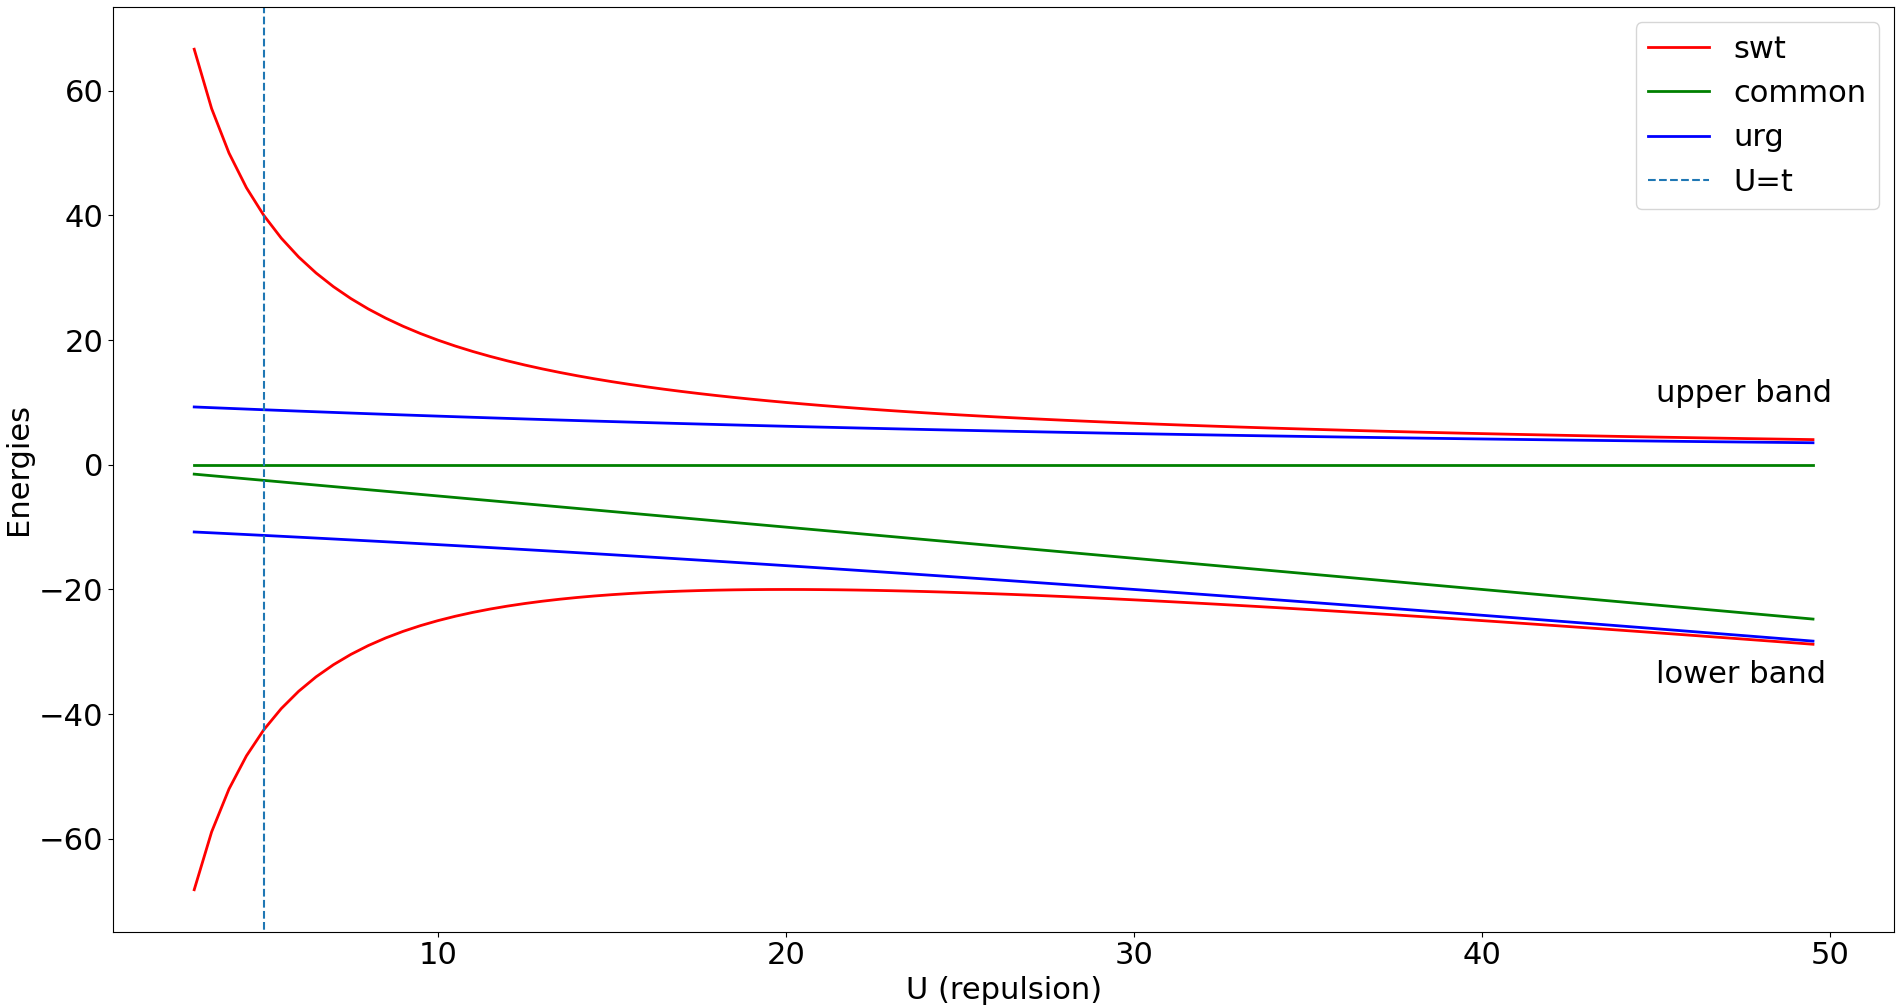
\includegraphics[width=\textwidth]{./com_plot}}
\end{figure}

\section{Effective Hamiltonian}
The goal is to obtain the unitary transformation. In the half-filled subspace for the Hubbard dimer,
\beq
\ham = \bordermatrix{~ & \ket{\ua,\da} & \ket{\ua\da,0} & \ket{\da,\ua} & \ket{0,\ua\da} \cr
	& 0 & t & 0 & -t \cr \\
	& t & U & -t & 0 \cr \\
	& 0 & -t & 0 & t\cr \\
	& -t & 0 & t & U \cr}
\eeq
I have dropped the part of the Hamiltonian involving \il{\ket{\ua,\ua}} and \il{\ket{\da,\da}} because they are already decoupled and do not change under the RG. Notice that \il{\ham} can be written as 
\beq
	\ham = \bordermatrix{~ & \ket{n_{1\ua} = 1} & \ket{n_{1\ua}=0} \cr
		& a & b \cr\\
		& b & a \cr}
\eeq
Applying RG on this matrix,
\begin{gather}
H_e = H_h = a \\
T = b\\
\eta^\dagger = \fr{1}{E - H_e}c^\dagger_{1\ua} T = \fr{1}{E - a}c^\dagger_{1\ua}b\\
\implies \eta  = b^\dagger c_{1\ua}\fr{1}{E - a}
\end{gather}
From properties of \il{\eta},
\begin{gather}
\hat n_{1\ua} = \eta^\dagger \eta = \fr{1}{E-a}c^\dagger_{1\ua}c_{1\ua}bb^\dagger\fr{1}{E-a} \\
\implies(E-a)^2 \hat n_{1\ua} = \hat n_{1\ua}b^2
\end{gather}
I used \il{b = -t\sigma_x \implies b^\dagger = b}. The two solutions for \il{E} are
\begin{gather}
E -a = \pm b \\
\implies E_\pm = a \pm b\\
\implies \ham_\text{rotated} = \bordermatrix{~ & \ket{n_{1\ua} = 1} & \ket{n_{1\ua}=0} \cr
		& a-b & 0 \cr
		& 0 & a+b \cr}
		=\begin{pmatrix}
		  0 & 2t & 0 & 0 \\
		  2t & U & 0 & 0 \\
		  0 & 0 & 0 & 0 \\
		  0 & 0 & 0 & U
	  \end{pmatrix}
\end{gather}
For this step, the unitary is
\beq
U_1 = \fr{1}{\sqrt 2} \bordermatrix{~ & \ket{n_{1\ua} = 1} & \ket{n_{1\ua}=0} \cr
				      & -1 & 1 \cr\\
				      & 1 & 1 \cr}
	= \fr{1}{\sqrt 2} \begin{pmatrix} \\ & -\mathbb{I}_{2\times 2} & \mathbb{I}_{2\times 2} &\\\\\\
	& \mathbb{I}_{2\times 2} & \mathbb{I}_{2\times 2} & \\
	&&&
	\end{pmatrix}
\eeq
Taking a look at \il{\ham_\text{rotated}}, the lower block is diagonal. So, take the upper block as the new Hamiltonian,
\begin{gather}
\ham = \bordermatrix{~ &  \ket{0,\da} & \ket{\da,0}\cr
	     & 0 & 2t \cr
	     & 2t & U \cr}\\
H_e = 0, H_h = U, T = 2t \\
\eta^\dagger = \fr{1}{E - H_e} c_{1\da}^\dagger T = \fr{2t}{E} c_{1\da}^\dagger \\
\eta = \fr{1}{E - H_h} T^\dagger c_{1\da} = \fr{2t}{E - U} c_{1\da}\\
\hat n_{1\da} = \eta^\dagger \eta = \fr{4t^2}{E(E-U)}\hat n_{1\da}\\
\implies E(E-U)=4t^2 \implies E = \fr{U\pm\Delta}{2}
\end{gather}
Therefore,
\begin{gather}
	\ham_{rotated} = \begin{pmatrix}\fr{U-\Delta}{2} & 0 \\ 0 & \fr{U+\Delta}{2} \end{pmatrix}\\
	\mathcal{U} = \begin{pmatrix} \fr{4t}{U-\Delta} & \fr{4t}{U+\Delta} \\ 1 &1 \end{pmatrix}
	\end{gather}
\il{N_\pm^2 = \Delta\rr{\Delta\pm U}}. Since this unitary acts only on the upper block, the complete unitary for this stage is
\beq
		U_2 = \begin{pmatrix} \mathcal{U} & 0_{2\times 2} \\
		0_{2\times 2} & \mathbb{I}_{2\times 2}\end{pmatrix}
\eeq
The total unitary for the entire diagonalization process is
\beq
U = U_1 \times U_2 = \fr{1}{\sqrt 2}\begin{pmatrix}
	-\mathcal{U} & 1 \\
	\mathcal{U} & 1
	\end{pmatrix}
\eeq
To check whether these are correct, we can compute the eigenstates. The eigenstates of the unitarily rotated Hamiltonian are just the fermionic degrees of freedom \il{\ket{n_{i\sigma}}}. The eigenstates of the bare Hamiltonian are hence obtained by rotating these states:
\beq
			\overline {\ket{\psi_1}}=U\ket{\ua,\da} = \fr{1}{\sqrt 2}\begin{pmatrix} -\mathcal{U} & 1 \\& \\ 
				\mathcal{U} & 1 \end{pmatrix} \begin{bmatrix} 1 \\ 0 \\ 0 \\ 0 \end{bmatrix} &= \fr{1}{\sqrt 2}\begin{bmatrix} -\fr{4t}{U-\Delta} \\ -1 \\ \fr{4t}{U-\Delta} \\ 1 \end{bmatrix} \sim \fr{1}{\sqrt 2}\cc{\fr{4t}{U-\Delta}\rr{\ket{\ua,\da} - \ket{\da,\ua}}+\rr{\ket{\ua\da,0}-\ket{0,\da\ua}}}\\
				\overline {\ket{\psi_2}}=U\ket{\ua,\da} &=  \fr{1}{\sqrt 2}\begin{bmatrix} -\fr{4t}{U+\Delta} \\ -1 \\ \fr{4t}{U+\Delta} \\ 1 \end{bmatrix} \sim \fr{1}{\sqrt 2}\cc{\fr{4t}{U+\Delta}\rr{\ket{\ua,\da} - \ket{\da,\ua}}+\rr{\ket{\ua\da,0}-\ket{0,\da\ua}}} \\
				\overline {\ket{\psi_3}}=U\ket{\ua,\da} &=  \begin{bmatrix} 1 \\ 0 \\ 1 \\ 0 \end{bmatrix} \sim \fr{1}{\sqrt 2}\rr{\ket{\ua,\da} + \ket{\da,\ua}}\\
				\overline {\ket{\psi_4}}=U\ket{\ua,\da} &= \begin{bmatrix} 0 \\ 1 \\ 0 \\ 1 \end{bmatrix} \sim \fr{1}{\sqrt 2}\cc{\ket{\ua\da,0} + \ket{0,\ua\da}}
\eeq
Now that we have the unitary transformaiton, the contention is that the following is the correct effective Hamiltonian:
\beq
\overline \ham = U\hat n_{2\ua}\hat n_{2\da} + \fr{U-\Delta}{2}\hat n_{1\ua}\hat n_{2\da}+ \fr{U+\Delta}{2}\hat n_{1\ua}\hat n_{1\da}
\eeq
\subsubsection*{Matching eigenvalues}
To check that this gives the correct eigenvalues, I operate this on the states which should be its eigenstates, that is, the decoupled degrees of freedom \il{\ket{n_{i\sigma}}}:
\beq
\ol \ham \ket{\ua,\da}&=\begin{pmatrix} \fr{U-\Delta}{2} & 0 & 0 & 0 \\ 0 & \fr{U+\Delta}{2} & 0 & 0 \\ 0 & 0 & 0 & 0 \\ 0 & 0 & 0 & U \end{pmatrix}\begin{bmatrix} 1 \\ 0 \\ 0 \\ 0 \end{bmatrix} = \fr{U-\Delta}{2}\\
\ol \ham \ket{\ua\da,0}&=\begin{pmatrix} \fr{U-\Delta}{2} & 0 & 0 & 0 \\ 0 & \fr{U+\Delta}{2} & 0 & 0 \\ 0 & 0 & 0 & 0 \\ 0 & 0 & 0 & U \end{pmatrix}\begin{bmatrix} 0 \\ 1 \\ 0 \\ 0 \end{bmatrix} = \fr{U+\Delta}{2}\\
\ol \ham \ket{\da,\ua}&=\begin{pmatrix} \fr{U-\Delta}{2} & 0 & 0 & 0 \\ 0 & \fr{U+\Delta}{2} & 0 & 0 \\ 0 & 0 & 0 & 0 \\ 0 & 0 & 0 & U \end{pmatrix}\begin{bmatrix} 0 \\ 0 \\ 1 \\ 0 \end{bmatrix} = 0\\
\ol \ham \ket{0,\ua\da}&=\begin{pmatrix} \fr{U-\Delta}{2} & 0 & 0 & 0 \\ 0 & \fr{U+\Delta}{2} & 0 & 0 \\ 0 & 0 & 0 & 0 \\ 0 & 0 & 0 & U \end{pmatrix}\begin{bmatrix} 0 \\ 0 \\ 0 \\ 1 \end{bmatrix} = U\\
\eeq
Next is a proof that \il{\ol \ham} is unitarily linked with the bare Hamiltonian by the same unitary transformation:
\beq
U \overline \ham U^{-1} = U	\begin{pmatrix} \fr{U-\Delta}{2} & 0 & 0 & 0 \\ 0 & \fr{U+\Delta}{2} & 0 & 0 \\ 0 & 0 & 0 & 0 \\ 0 & 0 & 0 & U \end{pmatrix} U^{-1} = \begin{pmatrix}
	0 & t & 0 & -t  \\
	t & U & -t & 0  \\
	0 & -t & 0 & t \\
-t & 0 & t & U \end{pmatrix} = \ham
\eeq
This proves that \il{\overline \ham} shares the symmetries of \il{\ham}.\\\\

\subsubsection*{Rotated spin-inversion operator}
The spin-inversion operator in the original basis is
\beq
T = \begin{pmatrix} 0 & 0 & 1 & 0 \\ 0 & -1 & 0 & 0\\ 1 & 0 & 0 & 0\\0& 0 & 0 & -1 \end{pmatrix} = \begin{pmatrix} a & a + \mathbb{I} \\ a + \mathbb{I} & a \end{pmatrix}
\eeq
where \il{a = \begin{pmatrix} 0 & 0 \\ 0 & -1 \end{pmatrix}}.
To see the nature of the rotated spin-inversion operator,
\beq
	\ol{T} = U^{-1} T U = \begin{pmatrix} -\mathbb{I} & 0 \\ 0 & \sigma_z \end{pmatrix}
\eeq
To see that \il{\ol T} commutes with \il{\ol H},
\beq
\bar T \bar H &= \begin{pmatrix}-\mathbb{I} & 0 \\ 0 & \sigma_z \end{pmatrix}\begin{pmatrix} \fr{U-\Delta}{2} & 0 & 0 & 0 \\ 0 & \fr{U+\Delta}{2} & 0 & 0 \\ 0 & 0 & 0 & 0 \\ 0 & 0 & 0 & U \end{pmatrix}  = \begin{pmatrix} -\fr{U-\Delta}{2} & 0 & 0 & 0 \\ 0 & -\fr{U+\Delta}{2} & 0 & 0 \\ 0 & 0 & 0 & 0 \\ 0 & 0 & 0 & -U \end{pmatrix}\\
\bar H \bar T &= \begin{pmatrix} \fr{U-\Delta}{2} & 0 & 0 & 0 \\ 0 & \fr{U+\Delta}{2} & 0 & 0 \\ 0 & 0 & 0 & 0 \\ 0 & 0 & 0 & U \end{pmatrix}  \begin{pmatrix}-\mathbb{I} & 0 \\ 0 & \sigma_z \end{pmatrix} = \begin{pmatrix} -\fr{U-\Delta}{2} & 0 & 0 & 0 \\ 0 & -\fr{U+\Delta}{2} & 0 & 0 \\ 0 & 0 & 0 & 0 \\ 0 & 0 & 0 & -U \end{pmatrix}
\eeq

\subsection*{Entanglement}
\beq
\ket{GS} = \fr{1}{\sqrt{2\rr{1+\alpha^{-2}}}}\qq{\ket{\ua,\da}-\ket{\da,\ua} +\alpha^{-1}\rr{\ket{0,\ua\da} - \ket{\ua\da,0}}}
\eeq
To determine the entanglement between the two states, I compute the von Neumann entropy of the reduced density matrix of the site 1 obtained by tracing out site 2.
\beq
\rho &= \ket{GS}\bra{GS}\\
\rho_1 &= \sum_{\ket{x}_2}\bra{x}\rho\ket{x}
\eeq
where the sum is over all the configurations of the second site: \il{\{\ket{x}\} = \{\ket{0},\ket{\ua},\ket{\da},\ket{\ua\da}\}}
\beq
\bra{0}_2 \rho \ket{0}_2 &= \fr{\alpha^{-2}}{2(1+\alpha^{-2})}\ket{\ua\da}\bra{\ua\da}\\
\bra{\ua}_2 \rho \ket{\ua}_2 &= \fr{1}{2(1+\alpha^{-2})}\ket{\da}\bra{\da}\\
\bra{\da}_2 \rho \ket{\da}_2 &= \fr{1}{2(1+\alpha^{-2})}\ket{\ua}\bra{\ua}\\
\bra{\ua\da}_2 \rho \ket{\ua\da}_2 &= \fr{\alpha^{-2}}{2(1+\alpha^{-2})}\ket{0}\bra{0}\\
\eeq
Therefore,
\beq
\rho_1 &= \fr{1}{2(1+\alpha^{-2})}\qq{\ket{\ua}\bra{\ua}+ \ket{\da}\bra{\da} + \alpha^{-2}\rr{\ket{\ua\da}\bra{\ua\da} + \ket{0}\bra{0}}}\\
       &=\fr{1}{2(1+\alpha^{-2})}\begin{pmatrix}1 & & & \\ & 1 & & \\ & & \alpha^{-2} & \\ & & & \alpha^{-2} \end{pmatrix}
\eeq
The von Neumann entropy is given by \il{S_1 = -\sum_i \lambda_i \log \lambda_i}, where \il{\lambda_i} are the eigenvalues.
\beq
S &= -\fr{1}{2(1+\alpha^{-2})}\times 2 \times \qq{\ln \fr{1}{2(1+\alpha^{-2})} + \alpha^{-2}\ln \fr{\alpha^{-2}}{2(1+\alpha^{-2})}}\\
  &=\fr{1}{(1+\alpha^{-2})}\qq{\ln \rr{2+2\alpha^{-2}} + \alpha^{-2}\ln \rr{2+2\alpha^{2}}}
\eeq
\begin{center}
	\includegraphics*[scale=0.4]{S1.png}
\end{center}
The entropy is maximum (\il{\log 4}) at \il{\fr{U}{4t} = 0} and minimum (\il{\log 2}) at \il{\fr{U}{4t} \ra \infty}. This is expected for the following reason: At \il{U = 0}, the ground state becomes an equal admixture of all four states. If a measurement is performed on site 2, site 1 ends up in any one of the four possible configurations (\il{\ket{0},\ket{\ua},\ket{\da},\ket{\ua\da}}), with equal probability. The fact that the probabilities are equal means the resultant state will be maximally entangled, which leads to the entropy taking the form \il{\log N}, where \il{N} is the dimension of the reduced Hilbert space. Since site 1 can go into four possible states,  the value of \il{N}  is 4, and we get \il{S_1 = \log 4}.\\\\
For \il{U=\infty}, the ground state is just a singlet (\il{\ket{\ua,\da} - \ket{\da,\ua}}), that is, an equal admixture of two states. This means that on measuring site 2, site 1 now has only two options to choose from, \il{\ket{\ua}} or \il{\ket{\da}}, the doublon-holon states are out of the picture. This reduces the dimension of the available Hilbert space to 2, and we get \il{\log 2}.

To find the entanglement content of just the singlet part, I can project out the doublon-holon part from the density matrix.
\beq
\rho_{sg} = \fr{1}{2}\begin{pmatrix}1 & 0 \\ 0 & 1 \end{pmatrix}
\eeq
The entropy will just be \il{\log 2}. Projecting out the singlet part and keeping the doublon-holon part will give the same entropy.

\end{document}
